

%----------------------------------------------------------------------------------------
%	PART
%----------------------------------------------------------------------------------------




\part{Ejercicios}
\graphicspath{ {A_Capitulo_Ejercicios/img/ejemplos/}, {W_Varios/2_Portada_capitulos} }

%----------------------------------------------------------------------------------------
%	Ejercicios
%----------------------------------------------------------------------------------------

\chapterimage{A_Capitulo_Ejercicios/img/portada/ima2} % Chapter heading image

\chapter {Ejercicios}

\addcontentsline{toc}{chapter}{\textcolor{ocre}{Capítulo 1}}


\begin{itemize}
 \item 1. Calcular el interés simple 300.000 COP desde el 18 de marzo al 18 de junio del mismo año al 3,4\% periodo mes vencido.\\
       \textbf{Respuesta:} COP 30.600
       \medskip

 \item 2. Una persona invierte COP 250.000 al 40\% "nominal anual año vencido" desde el 15 de septiembre de 1998 hasta el 18 de noviembre de 1998. Calcular:
       \\
       a) el valor final racional y
       b) el valor final bancario.
       \\
       \textbf{Respuestas:} a) COP 267.534,25  b) COP 2'677.777,78
       \medskip

 \item 3. ¿Cuánto debe invertirse hoy 17 de octubre en un fondo que garantiza el 28\% "nominal anual año vencido" para que el 20 de marzo del siguiente año pueda retirar la suma de COP 150.000?\\
       \textbf{Respuesta:} COP 134.151,72
       \medskip


 \item 4. Hallar el valor presente de COP 500.000 en 3 y 1/2 años al 3\%período mes vencido\\
       \textbf{Respuesta:} COP 221.239
       \medskip

 \item 5. Hace 6 años compré un lote en COP 900.000 y hoy se vendió en COP 6 millones. Hallar la tasa de interés "nominal anual año vencido" comercial que gané en este negocio.\\
       \textbf{Respuesta: }94,44\% "nominal anual año vencido"
       \medskip

 \item 6. ¿Qué tan rentable es un documento que hoy se puede comprar en COP 750.000 el cual devolverá al cabo de 3 años la suma de COP 3'300.000?\\
       \medskip

 \item 7. Se recibe un préstamo por  COP  1 millón al 42\% nominal anual año vencido el día 8 de agosto de 1999 con vencimiento el 8 de marzo del 2000. Hallar el valor final del préstamo calculando los intereses (I):\\

       a) interés exacto o racional\\
       b) interés comercial o base 360\\
       e) interés bancario\\
       d) interés base 365\\
       Tenga en cuenta que el año 2000 es un año bisiesto\\
       \textbf{ Respuestas:} a) COP 1'244.426,23; b) COP 1'245.000; e) COP 1'248.500; d) COP 1'243.945,21
       \medskip

 \item 8. Un pagaré con valor presente de  COP  300.000 emitido el 15 de septiembre de 1999 con plazo de 270 días a una tasa de interés del 30\% nominal anual año vencido.\\
       Hallar el valor futuro y la fecha de vencimiento en:\\

       a) interés exacto o racional\\
       b) interés comercial o base 360\\
       c) interés bancario\\
       d) interés base 365\\
       \textbf{Respuestas:} a) COP 366.393,44; 11-06-00; b) COP 367.500; 15-06-00; c) COP 367.500; 11-06-00; d) COP 366.575,34; 12-06-00
       \medskip

 \item 9. Una letra por COP 550.000 madura el 23 de agosto de 1998 y va a ser descontada el 17 de julio del mismo año al 38\% "nominal anual año vencido". Determinar el valor de la transacción.\\
       \textbf{Respuesta:} COP 528.519,44
       \medskip

 \item 10. El 15 de diciembre de 1999 una empresa recibe un pagaré por  COP  2 millones a un plazo de 3 meses al 25\% nominal anual año vencido de interés comercial simple. El 14 de enero lo negocia con un banco que lo adquiere a una tasa de descuento del 29\% nominal anual año anticipado en interés bancario. ¿Cuánto recibirá la empresa por el pagaré y cuánto ganará el banco en la operación de descuento?\\

       \textbf{Respuestas:} la empresa recibe COP 2.020.579,86; el banco gana COP 104.420,14
       \medskip

 \item 11. Halle el valor de maduración de un pagaré con vencimiento el 20 de abril si va a ser descontado el 13 de marzo del mismo año al 40\% "nominal anual año vencido" y su valor de transacción es de  COP  780.400\\
       \medskip

 \item 12. Una persona solicita un préstamo a un banco por la suma de COP 800.000, a un plazo de 90 días y le cobran una tasa anticipada del 38\% "nominal anual año vencido".\\

       a) ¿Cuál es el valor líquido que le entregan?\\
       b) Suponga que el banco cobra COP 15 000 por el estudio del crédito, ¿cuál será el valor liquido?\\

       \textbf{Respuestas:} a) COP 724.000; b) COP 709.000
       \medskip

 \item 13. ¿Cuál es el valor del documento que queda en poder de un banco, si el prestatario recibe un valor liquido de  COP 500.000 por un documento con maduración en 90 días, si le cobran una tasa de descuento del 41\% "nominal anual año vencido"? \\

       a) Sin tener en cuenta costos de apertura del crédito y\\
       b) Teniendo en cuenta que el banco cobra COP 2 000 por estudio del documento \\
       \medskip

 \item 14. Un documento de valor inicial COP 700.000 es fechado el 25 de septiembre de 1998 a un plazo de 325 días y un interés del 32\% "nominal anual año vencido". Si es descontado por un banco el 18 de marzo de 1999 al 40\% "nominal anual año vencido" determinar:\\

       a) La fecha de vencimiento\\
       b) El valor al vencimiento\\
       c) El valor de transacción \\
       Usar interés bancario\\

       \medskip

 \item 15. Hallar la verdadera tasa bancaria que cobra un banco cuando descuenta un documento con valor de maduración de COP 400.000 si es descontado 25 días antes del vencimiento al 41\% nominal anual año anticipado.\\

       \textbf{Respuesta:} 42,2\% nominal anual año vencido
       \medskip

 \item 16. Un almacén ofrece los siguientes descuentos, sobre una mercancía cuyo costo inicial es de COP 200.000:\\

       30\% por venta al por mayor, 10\% por pago al contado y 5\% por enviar la mercancía sin empaque.\\

       a)¿Cuál es el valor final de la factura?\\
       b) ¿Cuál es el descuento promedio que se otorgó?\\

       \textbf{Respuestas:} a) COP 119.700 b) 40,15\%
       \medskip

 \item 17. Una fábrica ofrece un descuento del 25\% en ventas al por mayor, el 5\% por pronto pago y el 4\% por embalaje. ¿Cuál debe ser el descuento adicional que puede ofrecerse a los empleados de la misma fábrica para que el descuento total no sea superior al 35\%?\\
       \textbf{Respuesta:} 4,971%\
       \medskip

 \item 18. Se compra un artículo por COP 870.000 el día 25 de noviembre y se acuerda que será cancelado mediante el sistema de pagos parciales, con un plazo máximo de 3 meses. Si el día de la compra se da una cuota inicial del 30\%, el 12 de diciembre se hace un abono parcial de COP 200.000 y el 20 de enero del siguiente año se hace otro abono parcial de COP 150.000 ¿cuál debe ser el valor del pago final que hecho al vencimiento cancelará la deuda? Suponga que se carga un interés bancario del 34\% "nominal anual año vencido".\\

       \textbf{Respuesta:} COP 293.865,71
       \medskip

\end{itemize}

\chapter*{Capítulo 2}
\addcontentsline{toc}{chapter}{\textcolor{ocre}{Capítulo 2}}


\begin{itemize}

 \item 1.	Se invierten 350.000 COP en un depósito a término fijo de 3 años al 28\% nominal anual trimestre vencido. Determinar el monto de la entrega al vencimiento del documento.  \\
       \medskip

 \item 2. Hallar el monto de 480.000 COP en 127 días suponiendo una tasa del 30\% "nominal anual año vencido", use un año de 360 días.\\
       \medskip

 \item 3.¿Qué capital debo invertir hoy para poder retirar un millón de pesos dentro de 18 meses suponiendo que el capital invertido gana el 28\%  nominal anual semestre vencido ?\\

       \textbf{Respuestas:}  674.971,52 COP
       \medskip

 \item 4. ¿Cuál es el valor presente de 800.000 COP en 36 días al 32\% "nominal anual año vencido"? Use un año de 360 días.\\
       \textbf{Respuestas:}  778'094,92 COP
       \medskip

 \item 5. Halle la rentabilidad anual de un documento que se adquiere en 300.000 COP y se vende 6 meses más tarde en 500.000 COP. \\
       \medskip

 \item 6. ¿A qué tasa nominal anual mes vencido se duplica un capital en 2,5 años?  \\
       \textbf{Respuestas:} 2,34\% nominal anual mes vencido
       \medskip

 \item 7. ¿A qué tasa nominal trimestral se triplica un capital en 4 años?\\
       \textbf{Respuestas:} 28,43\% nominal anual trimestre vencido
       \medskip

 \item 8. Una compañía dedicada a la intermediación financiera desea hacer propaganda para captar dineros del público, la sección de mercadeo le dice al gerente de la compañía que una buena estrategia de mercado es duplicar el dinero que depositen los ahorradores. Si la junta directiva de la compañía autoriza pagar por la captación de dinero un máximo de 2,5\% nominal anual mes vencido. ¿Cuánto tiempo debe durar la inversión?  \\
       \textbf{Respuestas:} 28,07 meses
       \medskip

 \item 9. ¿En cuánto tiempo se triplica un capital al 8\% periódico trimestral, sabiendo que el interés solo se paga por trimestres completos?\\
       \textbf{Respuestas:} 15 meses
       \medskip

 \item 10. Decidir la mejor alternativa entre invertir en una compañía de financiamiento comercial que en depósitos a término fijo paga el 28\% nominal trimestral vencido, o invertir en una empresa de turismo que garantiza triplicar el capital en 3 años y 6 meses.\\
       \textbf{Respuestas:} Es mejor la empresa de turismo
       \medskip

 \item 11. Una máquina que actualmente está en uso llegará al final de su vida útil  al final de 3 años, para esa época será necesario adquirir una nueva máquina y se estima costará unos US COP 2'000.000, la máquina que actual opera para esa época podrá ser vendida en 500.000 COP. Determinar el  valor que se debe depositar hoy en un depósito a término fijo de 3 años que garantiza el 7,5\% nominal anual año vencido  \\
       \medskip

 \item 12. a) Hallar una tasa nominal anual trimestre vencido equivalente al 7\% nominal anual trimestre vencido anticipado.\\
       \textbf{Respuestas:} a) 7,527\% nominal anual trimestre vencido \\

       b) Hallar una tasa nominal mensual anticipada equivalente al 3\% efectivo mensual. \\
       \textbf{Respuestas:} b) 2,913\% período mes anticipado
       \medskip

 \item 13. a. Hallar una tasa nominal anual semestre vencido equivalente al 24\% nominal anual trimestral vencido.\\
       \textbf{Respuestas:} a) 24,72\% nominal anual semestre vencido\\

       b. Hallar una tasa nominal anual trimestre anticipado equivalente al 2,5\% periódo mes vencido.\\
       \textbf{Respuestas:} b) 28,56\% nata
       \medskip

 \item 14.  a. Hallar una tasa mensual efectiva anticipada equivalente al 41,12\% nominal anual año vencido.\\
       \textbf{Respuestas:} a) 2,83\% nama \\

       b. Hallar una tasa nominal anual mes vencido equivalente al 36\% nominal anual mes anticipado.\\
       \textbf{Respuestas:} b) 3,093\% nominal anual mes vencido
       \medskip

 \item 15. a) Dado el 28\% nominal anual trimestre anticipado hallar una tasa nominal semestral equivalente.\\
       \textbf{Respuestas:} a) 31,24\% nominal anual semestre vencido \\

       b. Dado el 27\% nominal anual semestre vencido hallar una tasa nominal anual mes anticipado equivalente.\\
       \textbf{Respuestas:} a) 25,061\% nominal anual mes anticipado
       \medskip

 \item 16. a) Hallar una tasa efectiva anual, equivalente al 25\% nominal anual año vencido anticipado.\\
       \textbf{Respuestas:} a) i = 33,33\% nominal anual año vencido\\

       b) Hallar una tasa efectiva anual anticipada, equivalente al 36\% anual efectivo. \\
       \textbf{Respuestas:} b) $j_{a}$ = 26,47\% nominal anual año vencido\\

       c) Hallar una tasa efectiva anual anticipada, equivalente al 2,5\% periódo mes vencido.\\
       \textbf{Respuestas:} c) $j_{a}$ = 25,64\% nominal anual año vencido
       \medskip

 \item 17. Dado el 15\% periódo semestre vencido hallar una tasa equivalente para un quinquenio.\\
       \textbf{Respuestas:} 304,56\% (período 5 años) na5av
       \medskip

 \item 18. Dado el 208\% período 3 años hallar una tasa periódica equivalente para 2 años.\\
       \textbf{Respuestas:} 111.69\% (período 2 años)  p2av
       \medskip

 \item 19. Dado el 31\% nominal anual 205 días vencido (205 días vencido) hallar una tasa efectiva equivalente anual. Base 365 días.\\
       \textbf{Respuestas:} 33.08079\% nominal anual año vencido
       \medskip

 \item 20. Dado el 40\% nominal anual 185 días vencido (185 días vencido) hallar una tasa efectiva equivalente anual. Base 365 días.\\
       \textbf{Respuestas:} 43.9383467\% nominal anual año vencido
       \medskip

 \item 21. Dado el 35\% nominal anual 160 días vencidio (160 días vencido) hallar una tasa nominal anual 300 días vencido (300 días vencido) equivalente. Base 365 días.\\
       \textbf{Respuestas:} 37.3349\% nominal anual 300 días vencido (300 días vencido)
       \medskip

 \item 22. Dado el 43\% nominal anual 200 días vencido (200 días vencido) hallar una tasa nominal anual 111 días vencido (111 días vencido) equivalente.\\

       a) Base 360 días\\
       b) Base 365 días\\

       \textbf{Respuestas:} a)53,05304\% nominal anual 111 días vencido (111 días vencido), b)52,8799\% nominal anual 111 días vencido (111 días vencido)
       \medskip

 \item 23. Dado el 32\% nominal anual año vencido hallar la tasa nominal 158 días vencidos. \\
       \textbf{Respuestas:} a) 29,500356\% nominal anual 158 días vencido (158 días vencido)
       \medskip

 \item 24. Una persona tiene dos deudas una de 250.000 COP pagadera en 3 meses y otra de 400.000 COP pagadero en 7 meses. Si desea cambiar la forma de cancelarlas mediante dos pagos iguales de X COP c/u con vencimiento en 5 meses y 12 meses respectivamente, determinar el valor de los pagos suponiendo una tasa del 36\% nominal anual mes vencido.\\
       \medskip

 \item 25. Una empresa tiene dos deudas con un banco, la primera deuda es de 100.000 COP con interés del 30\% nominal anual mes vencido, se adquirió hace 6 meses y hoy se vence; la segunda por 200.000 COP al 32\% nominal anual mes vencido se contrató hace 2 meses y vence en 4 meses, debido a la incapacidad de cancelar la deuda, la empresa propone al banco refinanciar su deuda, llegándose a un acuerdo entre las partes de la siguiente forma: Hacer 3 pagos iguales con vencimiento en 6 meses, 9 meses y 12 meses, con una tasa del 33\% nominal anual mes vencido. ¿cuál es el valor de cada pago?\\
       \textbf{Respuestas:} 138.452,64 COP
       \medskip

 \item 26. Un almacén va a ser vendido el 20 agosto. Los inventarios realizados el mismo 20 de agosto arrojaron el siguiente resultado:\\

       a)	En caja 80.000 COP\\
       b)	En bancos 250.000 COP\\
       c)	Cuentas por cobrar \\
       C1 cheque por 65.000 COP para el 30 de septiembre\\
       C2 depósito a término fijo de 6 meses por 235.000 COP e intereses al 28\% nominal anual mes vencido, la inversión se efectuó hace 3 meses.\\
       d)	Mercancías por 950.000 COP\\
       e)	Cuentas por pagar:\\
       D1 cheque por 150.000 COP para el 21 de septiembre\\
       D2 letra por 400.000 COP para el 18 de noviembre.\\

       Con un interés del 30\% nominal anual año vencido usando interés bancario determine el valor del almacén el día de la venta.\\
       \textbf{Respuestas:} 1'074.317 COP
       \medskip

 \item 27. Hoy se contrae una deuda por 500.000 COP con intereses al 30\% nominal anual trimestre vencido y vencimiento en 6 meses y hay una deuda por 800.000 COP contraida hace 3 meses con interés al 32\% nominal anual semestre vencido y vencimiento en 1 año. ¿En qué fecha deberá hacer un pago de 1'700.000 COP para cancelar las deudas suponiendo que el rendimiento normal del dinero es del 2,5\% período mes vencido?\\
       \textbf{ Respuestas:} 9,027 meses
       \medskip

 \item 28. Hallar el tiempo en que debe hacerse un pago de 300.000 COP, para cancelar dos deudas: una de 150.000 COP, con vencimiento en 6 meses y  otra de 150.000 COP con vencimiento en 26 meses. Suponga una tasa del 30\% nominal anual mes vencido.\\
       \textbf{Respuestas:} 1 año, 2 meses y 23 días
       \medskip

 \item 29. Resuelva el problema anterior suponiendo una tasa del 30\% nominal anual trimestre vencido.\\
       \textbf{Respuestas:} 1 año, 2 meses y 24 días
       \medskip

 \item 30. Se deben pagar: 800.000 COP en 3 meses, 1'000.000 COP en 10 meses y 900.000 COP en 15 meses y se van a cancelar en dos pagos el primero por 1'700.000 COP en 9 meses,  ¿en qué fecha deberá pagar 850.510,96 COP para saldar las deudas suponiendo que el dinero rinde el 8\% período vencido?
       \medskip

 \item 31. En el desarrollo de un proyecto hubo necesidad de una inversión inicial de 700.000 COP y se obtuvieron ingresos por 500.000 COP en 3 meses y 450.000 COP a los 10 meses. Hallar la rentabilidad nominal anual mes vencido que generó el proyecto?\\
       \medskip

 \item 32. Una empresa debe cancelar hoy 15 de febrero de 1998 una deuda por 700.000 COP con intereses del 30\% período trimestre vencido adquirida el 15 de agosto de 1997 y otra deuda por 1'000.000 COP obtenida el 15 de diciembre 1997 con vencimiento el 15 de junio 1998 a la misma tasa de la deuda anterior, ante la dificultad de la empresa para cancelar la deuda, el acreedor propone cancelar las deudas con un pago de 200.000 COP ahora y otro de 2'200.000 COP en 10 meses. ¿Cuál es la tasa de interés efectiva anual de refinanciación que se está cobrando?\\
       \medskip

 \item 33. Una empresa tiene tres deudas así:
       \begin{center}
        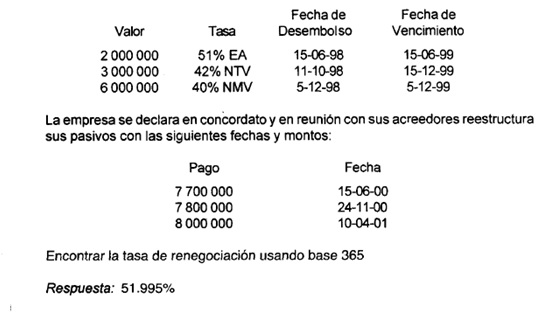
\includegraphics[height=9.2cm]{E2_33}
       \end{center}

\end{itemize}
\newpage


\chapter*{Capítulo 3}
\addcontentsline{toc}{chapter}{\textcolor{ocre}{Capítulo 3}}


\begin{itemize}

 \item 1. Se  constituye  un  CDT  a  180  días  por  COP 650.000,  con  una  tasa  del  26\% nominal anual trimestre vencido y teniendo  en  cuenta  que  la retención en la fuente es del 7\%"nominal anual año vencido" determinar:\\

       a. La tasa de interés(rentabilidad) antes de impuestos.\\
       b. La tasa de interés (rentabilidad) después de impuestos\\
       c. El valor en pesos que le entregan al vencimiento.\\
       d. Suponiendo una inflación del 18\% anual efectiva, determinar la tasa real obtenida.\\

       \medskip

 \item 2. Un inversionista desea  obtener  una  rentabilidad  real  del  8\%  "nominal anual año vencido" ¿A qué tasa periódica debe invertir suponiendo que la inflación va a ser del 18\% "nominal anual año vencido"?

       \textbf{Respuesta:} 27,44\% "nominal anual año vencido"\\
       \medskip

 \item 3. Un  artículo  es  fabricado  en  Estados  Unidos  y  se  vende  en  Colombia  en COP 500.000  ¿Cuánto  valdrá  el  artículo  en  Colombia  y  en  Estados  Unidos  al final  de  un  año,  suponiendo  los  siguientes  índices  económicos: cambio actual USD1 = COP 2.000, inflación en Estados Unidos 3\% "nominal anual año vencido", devaluación del peso 18\% "nominal anual año vencido"?\\
       \medskip

 \item 4. Un  artículo  es  fabricado en  Colombia  y  cuesta  COP 680.000,  cuando  el cambio es de USD1 = COP 2.000. Suponiendo que el IPP de este sector en Colombia es del 22\% "nominal anual año vencido", y que la devaluación del peso frente al dólar sea del 18\%"nominal anual año vencido", hallar el precio del mismo artículo en cada país al final de un año.\\
       \medskip

 \item 5. Dos  inversionistas  de  origen  alemán,  uno  residente  en  Alemania  y el  otro residente  en  Colombia,  han  decidido  realizar  un  negocio  en  Alemania  y cada uno aportará el 50\%. El negocio exige una inversión inicial de marcos  DMCOP 300 000   y   al   final   de   3   años   devolverá   la   suma   de   marcos DMCOP 400 000. Hallar las tasas totales y reales para cada uno de los socios suponiendo  que  los  siguientes  indicadores  económicos  se  mantuvieron estables durante los 3 años.\\

       a.tasa promedio de inflación en Colombia 22\% "nominal anual año vencido"\\
       b.tasa promedio de inflación en Alemania 2\% "nominal anual año vencido"\\
       c.   tasa  de  devaluación  del  peso  frente  al  dólar:  primer  año  18\% "nominal anual año vencido", segundo  año  20\% "nominal anual año vencido"  y  tercer  año  17\% "nominal anual año vencido",  devaluación  marco frente  al  dólar:  años  1  y  2  el  2\% "nominal anual año vencido",  para  el  tercer  año  hay  una revaluación del 3\% "nominal anual año vencido"\\
       d. cambio actual USCOP  = DMCOP 2,23               USCOP  = COP 1 300\\
       \medskip
       \textbf{Respuestas:} En marcos 10.06\% "nominal anual año vencido" y 7.9\% "nominal anual año vencido"; en pesos: 29,85\% "nominal anual año vencido" y 6,43\% "nominal anual año vencido".\\
       \medskip

 \item 6. El señor Yukimoto residente en el Japón y Mr.Jones residente en Estados Unidos  se  asocian para comprar un banco en Colombia, El valor de cada acción del banco es de COP 900.000 pesos/acción y esperan venderla al final de 3 meses en COP 900.700 pesos/acción. (Trabajar con 5 decimales).\\

       a. Cálcule la tasa de interés anual efectiva y la rentabilidad real(tasa de interés real) anual de cada uno de los socios\\
       b. ¿Cuánto tendrá cada uno en su respectiva moneda al final de los 3 meses?. Tome en cuenta la siguiente información:\\

       Inflación en: Colombia 18\% "nominal anual año vencido", en Estados Unidos 3.5\% "nominal anual año vencido", en Japón 2.3\%  "nominal anual año vencido" tasa de devaluación del peso frente al dólar 22\%  "nominal anual año vencido" tasa de devaluación del dólar frente al Yen 1\% "nominal anual año vencido" Cambio actual USCOP 1 = COP 2000; USCOP 1 = Yen105
      \medskip

 \item 7. Si en el problema anterior el valor del banco es de ochenta mil millones de pesos y Yukimoto  participa en el 40\% de la compra y Mr. Jones participa con el resto, determinar la cantidad que  recibirá c/u en su respectiva moneda.\\
      \medskip

 \item 8. En el país A cuya moneda es el ABC, un par de zapatos vale 240.000 de ABC, existe una inflación  del 22\%"nominal anual año vencido" y el cambio actual es de USCOP 1 = ABC 1.000. En el país X rige el dólar americano y se prevé  una inflación promedio del 6.5\% "nominal anual año vencido". Al final de un año ¿cuál debe ser la tasa de devaluación en A con respecto al dólar a fin de no perder competitividad en los mercados de X?\\
       \medskip

 \item 9. Un inversionista desea que todas sus inversiones le den una rentabilidad real del 5\% "nominal anual año vencido" ¿Qué  tasa anual efectiva debe ofrecérsela si la inflación esperada es del 17\%"nominal anual año vencido" de forma tal que satisfagan  los deseos del inversionista?
       \textbf{Respuesta:} 26.36\%"nominal anual año vencido"\\
       \medskip

 \item 10. Un ahorrador consigna en una corporación de ahorro y vivienda la suma de COP 300.000 el día 1 de  marzo y el día 20 de junio consigna COP 200.000.  ¿Cuánto  podrá  retirar  el  31  de  agosto  si la corporación  paga el  27\% "nominal anual año vencido" de corrección monetaria para los meses de marzo y abril y el 25\% "nominal anual año vencido"  para el resto del período (mayo, junio, julio y agosto).\\
       a. Elabore los cálculos en pesos\\
       b. Elabore los cálculos en UPAC sabiendo que el primero de marzo upac1 = COP 6 650\\
       \textbf{Respuestas:} COP 545 389 "nominal anual año vencido"\hspace{0,5cm} UPAC 73.1415\\
       \medskip

 \item 11. Se estima que la corrección monetaria del primer año será del 18\% "nominal anual año vencido" y la del segundo año del 17\% "nominal anual año vencido":\\
       a.Calcular la cantidad que antes de impuestos le entregarán a un inversionista que invierte la suma de COP 800.000 a dos años en una cuenta de ahorros en UPAC que le garantiza pagar la corrección monetaria más el 4\% "nominal anual año vencido" de interés sobre los UPAC.\\
       b. Calcule la rentabilidad (tasa de interés "nominal anual año vencido") obtenida antes de impúestos que el cambio actual es UPAC 1 = COP 14.000\\
       c. Si la retención en la fuente es del 7\% sobre los intereses, calcular la rentabilidad (tasa de interes "nominal anual año vencido") después de los impuestos\\
       d. Calcular la cantidad final que le entregarán después de impuestos\\
       \textbf{Respuestas:}a. COP 1'194 605.57 \hspace{0,5cm} b. 22.199\% "nominal anual año vencido"\hspace{0,5cm} c. 21,876\% "nominal anual año vencido"\hspace{0,5cm} d. COP 1'188 296.78\\
       \medskip

 \item 12. Hallar la tasa anual efectiva de;\\
       a. DTF +6 puntos\\
       b. IPC +7 puntos\\
       c Libor +8 puntos\\
       Asuma que: DTF = 15\% nata, IPC = 10\% nata, Libor = 5.14\% nominal anual semestre vencido\\
       \textbf{Respuestas:} a.24.07\% "nominal anual año vencido"\hspace{0,5cm} b.17.7\% "nominal anual año vencido"\hspace{0,5cm} c.13.57\% "nominal anual año vencido"\\
       \medskip

 \item 13. Suponiendo IPC = 8.5\% "nominal anual año vencido", CM= 12\% (CM= corrección monetaria), DTF = 15\% nata, TCC = 15.5\% nata, TBS (CF 180 días) = 19.27\% A.E., TBS(Bancos 360 días) = 19.19\% "nominal anual año vencido" Hallar X de las siguientes igualdades:\\
       \textbf{Observación:} TBS (CF 180 días) significa tasa básica del sector corporaciones financieras a 180 días.\\

       a. IPC+10 = CM+x\\
       b. CM+14 = TCC+X\\
       c. DTF +8.6 = IPC+X\\
       d. TBS(CF 180 días) + 6 = DTF+x\\
       e. TCC+3.5 = DTF+X\\
       f. IPC+4 = DTF+X\\
       \textbf{Respuestas:}a.6.56\% "nominal anual año vencido"\hspace{0,5cm} b.8.2\% nata "nominal anual año vencido"\hspace{0,5cm} c.17.55\%A.E
       \\d.7.775\% nata\hspace{0,5cm} e.4\% nata\hspace{0,5cm} f. -3.1\% nata\\
       \medskip

 \item 14. Asumiendo que $i_{dev}$  = 25\%, IPC = 9\% "nominal anual año vencido", Prime Rate = 8.25\% "nominal anual año vencido", DTF = 14.5\% nata, Libor = 5\% "nominal anual año vencido", resolver las siguientes ecuaciones:\\
       $i_{DEV}$  + 10 = IPC +X\\
       $i_{DEV}$  +(Prime+ 200 p.b.) = DTF +X\\
       $i_{DEV}$  + (Libor + 500 p.b.) = DTF +X\\
       \textbf{Respuestas:} a. 26.148\% "nominal anual año vencido"\hspace{0,5cm} "nominal anual año vencido". b. 16,32\% nata "nominal anual año vencido"\hspace{0,5cm} c, 16,11\% nata\\
       \medskip

 \item 15. ¿Cuál es la rentabilidad efectiva anual del comprador (tasa de interés "nominal anual año vencido") y el precio de compra para el que adquiere una aceptación financiera a 180 días si se conserva hasta su maduración, se registra en bolsa a un precio de 86.225\% y la comisión de compra es del 0.5\% "nominal anual año vencido" en rentabilidad?\\
       \textbf{Respuestas:} $i_{c} = 34\% "nominal anual año vencido"\hspace{0,5cm}  P_{c} = 86,37\%$\\
       \medskip

 \item 16. ¿Cuál es la comisión en pesos para el problema anterior suponiendo que la aceptación financiera tiene un valor nominal de COP 278.000?\\
       \textbf{Respuesta:} COP 450\\
       \medskip

 \item 17. ¿Cuál es la rentabilidad efectiva anual que obtiene un inversionista que adquiere en el mercado secundario una aceptación bancaria emitida a 90 días con un precio de registro de 97.254\% y le faltan 28 días para su maduración? Suponga una comisión de compra del 0.4\% "nominal anual año vencido" en rentabilidad. base 360.\\
       \textbf{Respuesta:} 42,645\% "nominal anual año vencido"\\
       \medskip

 \item 18. Un exportador recibe una aceptación bancaria por sus mercancías la cual vence en 180 días, tiene una tasa de emisión del 28\% nominal anual semestre vencido. El mismo día en que le entregan la aceptación la ofrece en bolsa. Si las comisiones de compra y de venta son de 0,4\% "nominal anual año vencido" y 0.6\% "nominal anual año vencido" respectivamente, calcular:\\
       a.La tasa de registro\\
       b.La tasa del comprador\\
       c.La tasa del vendedor\\
       d.El precio de registro\\
       e.El precio de compra\\
       \textbf{Respuestas:} a. 29.36\% "nominal anual año vencido"\hspace{0,5cm} b. 28.96\% "nominal anual año vencido"\hspace{0,5cm}  c. 29.96\% "nominal anual año vencido"\hspace{0,5cm} \\
       d. 87.922\% \hspace{0,5cm} e. 88.059\%.\\
       \medskip

 \item 19. Un inversionista compró el 14 de junio 98 una Aceptación Bancaria al 29.4\% "nominal anual año vencido" con vencimiento el 15 de mayo/99 por COP 250 millones, un segundo inversionista está dispuesto a adquirirlo el día 10 de septiembre/98 a una tasa del 34\% "nominal anual año vencido".\\
       a.¿Cuál será la utilidad en pesos del primer inversionista?\\
       b.¿Cuál es la rentabilidad del primer inversionista? (use un interés comercial es decir un año de 360 días).\\
       \textbf{Respuestas:} a. COP 7 598 455\hspace{1.0cm} b. 17.14\% "nominal anual año vencido"\\
       \medskip

 \item 20. Resuelva el problema anterior pero el segundo inversionista lo adquiere al 23.5\% "nominal anual año vencido"\\
       \textbf{Respuestaa:} a. COP 19 296 120\hspace{1,0cm} b. 47.8\% "nominal anual año vencido"\\
       \medskip

 \item 21. Suponga que el señor X posee una aceptación financiera con valor de vencimiento de COP 6 758.000 y desea venderla en Bolsa faltándole 57 días para vencerse y quiere ganarse un 29.5\% y la adquiere el señor Y. Suponga que la comisión de venta y de compra son 0.5\% "nominal anual año vencido" y 0. 47\% "nominal anual año vencido" respectivamente en rentabilidad. Base 365.\\
       a.¿Cuál es la tasa de registro?\\
       b.¿Cuál es el precio de registro?\\
       c. ¿Cuál la tasa que gana el señor Y?\\
       d.¿Cuál es el precio que paga el señor Y?\\
       e. ¿Cuál es la comisión de compra en pesos?\\
       \textbf{Respuestas:} a. $i_{R}= 29\%$"nominal anual año vencido"\hspace{0,5cm} b. $P_{R} = COP 6 494 534$\hspace{0,5cm}  c. $i_{c} = 28.53\%$ "nominal anual año vencido"\hspace{0,5cm}\\
       d. Pc= COP 6 498 237 \hspace{0,5cm} e. COP 3 703\\
       \medskip

 \item 22. El señor XX posee una aceptación bancaria por valor de COP 10 millones y la vende en Bolsa faltándole 87 días para su maduración, la adquiere el señor YY y el cual desea ganar el 32\% después de comisión pero antes de impuestos. Si la comisión de compra es del 0.4\% "nominal anual año vencido" y la de venta el 0.375\% "nominal anual año vencido" usando un año de 360 días determinar:\\
       a.	La tasa de registro\\
       b.	El precio de registro\\
       c.	La tasa de cesión\\
       d.	El precio de cesión\\
       e.	El precio al comprador\\
       f.	El valor en pesos de la retención en la fuente\\
       g.	La cantidad que debe pagar YY\\
       h.	La cantidad que recibe XX\\
       i.	La rentabilidad después de impuestos que gana YY\\
       \textbf{Respuestas:} a. $i_{R}$ = 32.4\% "nominal anual año vencido"\hspace{0,5cm}  b. $P_{R}$ = COP 9 344 234\hspace{0,5cm}   c. 32.775\% "nominal anual año vencido"\hspace{0,5cm}  \\
       d. COP 9 337 850\hspace{0,5cm}   e.  $P_{c}$ = COP 9 351 070;  "nominal anual año vencido"\hspace{0,5cm}    f. COP 45 904;  \hspace{0,5cm}   g. COP 9 396 974; \hspace{0,5cm}\\
       h. COP 9 383 754 \hspace{0,5cm} "nominal anual año vencido"\hspace{0,5cm}   i. 29.352\% "nominal anual año vencido".\\
       \medskip

 \item 23. En el problema 21 calcule el valor que recibe el vendedor y el valor que paga el comprador suponiendo que la retención en la fuente es del 7\% "nominal anual año vencido" sobre utilidades.\\
       \textbf{Respuestas:}\\
       El comprador paga COP 6 516 680,\\
       Vendedor recibe COP 6 509 055.\\
       \medskip

 \item 24. El 27 de abril de 1999 se compra una aceptación bancaria de COP 36 millones en el mercado bursátil, con vencimiento el 27 de julio de 1999 y con tasa de registro del 26\% "nominal anual año vencido". Si después de transcurridos 34 días la vende. ¿Qué precio se debe cobrar si el vendedor desea obtener una rentabilidad durante la tenencia del 26.5\% "nominal anual año vencido"?\\
       Base 365.\\
       \textbf{Respuesta}: $P_{v}$ = COP 34 736 688\\
       \medskip

 \item 25. Resuelva el problema anterior suponiendo que el corredor cobra una comisión del 0.1\% en rentabilidad y que de todas maneras el vendedor quiere ganarse el 26.6\% "nominal anual año vencido" durante la tenencia.\\
       \textbf{Respuesta:} $P_{v}$ =COP 34'746.123\\


\end{itemize}

%%%%%%%%%%%%%%%%%%%%%%%%%%%%%%%%%%%%%%%%%%%%%%%%%%%%%%%%%%%%%%%%%%%%%%%%%%%%%%%


\chapter*{Capítulo 4}
\addcontentsline{toc}{chapter}{\textcolor{ocre}{Capítulo 4}}


\begin{itemize}

 \item 1. Hallar el monto y el valor presente de 20 pagos de COP 200.000 c/u, suponga una tasa del 18\% "nominal anual año vencido".\\
       \medskip

 \item 2. Para la compra de un automóvil que vale COP 6 000 000; se exige una cuota inicial del 40\% y el resto se cancela en 36 cuotas mensuales, ¿a cuánto ascenderá la cuota, si los intereses son del 3.5\% período mes vencido\\
       \textbf{Respuesta:} COP 177.422,99\\
       \medskip

 \item 3. Si en el problema anterior se ofrecen 2 cuotas extraordinarias: la primera de
       COP 350.000 en el mes 5, y la segunda de COP 500.000, en el mes 18, ¿cuál será el valor de la cuota ordinaria?\\
       \textbf{Respuesta:} COP 149.633,07\\
       \medskip

 \item 4. Una persona va a comprar una máquina que vale COP800.000, con el objeto de poder disponer de esa cantidad el 15 de diciembre de 1989. Comienza a hacer depósitos mensuales de  COP  "R", en un fondo que paga el 30\% nominal anual mes vencido. Si el primer depósito lo hace el 15 de febrero de 1988, Hallar el valor del depósito mensual.\\
       \textbf{Respuesta:} COP26.157,10\\
       \medskip

 \item 5. Un documento estipula pagos trimestrales de COP100.000 iniciando el primer pago el 20 de enero de 1987 y terminando el 20 de julio de 1995: Si se desea cambiar este documento por otro que estipule pagos trimestrales de  COP  "R", comenzando el 20 de abril de 1988 y terminando el 20 de julio de 1989, Hallar el valor de la cuota. Suponga una tasa del 20\% nominal anual trimestre vencido. \textbf{Sugerencia}: El valor de los documentos debe ser igual en el punto que escoja como período focal.\\
       \medskip

 \item 6. Una persona se compromete a pagar COP600.000 mensuales, a partir del 8 de julio de 1988 hasta el 8 de diciembre de 1989. Se propone hacer depósitos mensuales de  COP  "R" c/u, en una cuenta de ahorros que como mínimo le garantiza el 1.5\% periódo mes vencido. Si el primer depósito lo efectúa el 8 de marzo de 1986, ¿cuál será el valor de  COP  "R" (valor de la serie uniforme), suponiendo que el último depósito lo hará:\\
       a, El 8 de diciembre de 1989\\
       b. El 8 de julio de 1988\\
       c. El 8 de junio de 1988\\
       d. El 8 de abril de 1987\\
       \medskip

 \item 7. Una deuda de COP 8'000.000 va a ser cancelado en pagos trimestrales de COP 780.000 durante tanto tiempo como fuere necesario. Suponiendo una tasa del 30\% nominal anual trimestre vencido.\\
       a. ¿Cuántos pagos de COP 780.000 deben hacerse?\\
       b. ¿Con qué pago final hecho 3 meses después del último pago de COP 780.000 cancelará la deuda?\\
       \medskip

 \item 8. Resuelva el problema anterior si la tasa es del 42\% nominal anual trimestre vencido. Justifique su respuesta desde el punto de vista matemático y desde el punto de vista financiero.\\
       \medskip

 \item 9. Desean reunirse exactamente COP 600.000 mediante depósitos mensuales de COP 10.000, en un fondo que paga el 36\% nominal anual mes vencido.\\
       a. ¿Cuántos depósitos de COP 10.000 deberán hacerse?\\
       b. ¿Qué depósito adicional hecho conjuntamente con el último depósito de COP 10.000 completará los COP 600.000?\\
       c. ¿Qué depósito adicional hecho un mes después del último depósito de COP 10.000 completará los COP 600.000?\\
       \medskip
 \item 10. Resolver el problema anterior incluyendo un depósito adicional de COP 70.000 en el período 10.\\
       \medskip

 \item 11. Para cancelar una deuda de COP 8'000.000, con intereses al 24\% nominal anual mes vencido se hacen pagos mensuales de COP 300.000 cada uno.\\
       a.¿Cuántos pagos de COP 300.000 deben hacerse?\\
       b.¿Con qué pago adicional hecho conjuntamente con el último pago de COP 300.000 se cancelará la deuda?\\
       c. ¿Qué pago adicional hecho un mes después del último pago de COP 300.000 cancelará la deuda?\\
       \medskip

 \item 12. Resolver el problema anterior suponiendo que se hace un pago adicional de COP 10.000 con la décima cuota.\\
       \medskip

 \item 13. Una máquina cuesta al contado COP 600.000, para promover las ventas, se ofrece que puede ser vendida en 24 cuotas mensuales iguales, efectuándose la primera el día de la venta. Si se carga un interés del 3\% período mes vencido . Calcular el valor de cada pago.\\
       \textbf{Respuesta:} COP 34.396,55\\
       \medskip

 \item 14. Un fondo para empleados presta a un socio la suma de COP 2 millones para ser pagado en 3 años, mediante cuotas mensuales uniformes, con intereses sobre saldos al 24\% nominal anual mes vencido. Si en el momento de pagar la sexta cuota, decide pagar en forma anticipada las cuotas 7, 8 y 9:\\
       a. ¿cuál debe ser el valor a cancelar al vencimiento de la sexta cuota?\\
       b. ¿cuál debe ser el valor de los intereses descontados?\\
       \textbf{Respuestas:} a. COP 304.751,66 \hspace{1,5cm}b. COP 9.111\\
       \medskip

 \item 15. Una  persona adopta un plan de ahorros del fondo ABC, que establece depósitos mensuales de COP 100.000, comenzando el primero de febrero de 1986 hasta el primero de abril de 1987 y, depósitos mensuales de COP 200.000, desde el primero de mayo de 1987 hasta el primero de diciembre de 1987. El capital así reunido permanecerá en el fondo hasta el primero de junio de 1988, fecha en la cual le será entregado al suscriptor junto con intereses calculados al 12\% nominal anual mes vencido. \\
       Por razones comerciales la junta directiva del fondo ABC decidió que, a partir del primero de octubre de 1986, el fondo pagará a todos sus clientes de ahorros el 18\% nominal anual mes vencido. ¿Cuál será el capital que, el primero de junio de 1988, le entregarán a la persona que ha decidido adoptar el plan?\\
       \medskip

 \item 16. Un contrato de arriendo por un año establece el pago de COP 200.000 mensuales al principio de cada mes. Si ofrecen cancelar todo el contrato a su inicio, ¿cuánto deberá pagar?. Suponiendo:\\
       a. tasa del 30\% nama (Nominal Anual mes anticipado).\\
       b. tasa 3\% período mes anticipado \\
       \medskip

 \item 17. Una máquina produce 2.000 unidades mensuales las cuales deben venderse a COP 80 c/u. El estado actual de la máquina es regular y si no se repara podría servir durante 6 meses más y luego desecharla, pero si hoy le hacemos una reparación total a un costo de COP 800.000, se garantizaría que la máquina podría servir durante un año contado a partir de su reparación. Suponiendo una tasa del 4\% período mes anticipado ¿será aconsejable repararla?\\
       \textbf{Respuesta:} No es aconsejable repararla\\
       \medskip

 \item 18. Elaborar una tabla para amortizar la suma de COP 3 millones en pagos trimestrales durante 15 meses con una tasa del 46\% nominal anual trimestre vencido.\\
       \textbf{Respuesta parcial:} Cuota t rimestralCOP 821.945,32 \\
       \medskip

 \item 19. Elaborar una tabla para capitalizar la suma de COP 2 millones mediante depósitos semestrales durante 3 años. Suponga una tasa del 42\% nominal anual semestre vencido\\
       \textbf{Respuesta parcial:} Depósito semestral COP 196.405,92 \\
       \medskip

 \item 20. Una persona desea reunir COP800.000 mediante depósitos mensuales de  COP  "R" c/u durante 5 años en una cuenta que paga el 30\% nominal anual mes vencido. ¿Cuál es el total de intereses ganados hasta el mes 30?\\
       \textbf{Respuesta:} COP81.785,81\\
       \medskip

 \item 21. Para cancelar una deuda de COP2 millones con intereses al 36\% nominal anual mes vencido se hacen pagos mensuales de  COP  "R" c/u, durante 15 años.\\
       a. Calcular el valor de la deuda después de haber hecho el pago número 110\\
       b. Calcular el total de los intereses pagados hasta el mes 110\\
       \textbf{Sugerencia:}para la parte a. calcule el valor presente en el mes 110  de los 70 pagos que falta por cancelar, para la parte b. halle la diferencia entre el total pagado y el total amortizado.
       \textbf{Respuestas:} a. COP 1'755.991,89 \hspace{1,5 cm} b. COP 6'388.423,79\\
       \medskip

 \item 22. Se necesita COP 1 millón, para realizar un proyecto de ampliación de una bodega, una compañía A ofrece prestar el dinero, pero exige que le sea pagado en 60 cuotas mensuales vencidas de COP 36.132,96 c/u. La compañía B ofrece prestar el dinero, pero para que le sea pagado en 60 pagos mensuales de COP 19.000 c/u y dos cuotas adicionales así: la primera de COP 250.000, pagadera al final del mes 12, la segunda, de COP 350.000, pagadera al final del mes 24. Hallar la tasa periódica mensual vencida que cobra cada uno, para decidir que préstamo debe utilizar.\\
       \textbf{Respuesta:} A. 3\% período mes vencido  \hspace{0,5 cm}              B. 2,35\% período mes vencido\\
       Utilice la compañía B.\\
       \medskip

 \item 23. Un equipo de sonido cuesta COP 4'000.000 al contado, pero puede ser cancelado en 24 cuotas mensuales de COP 330.000 c/u efectuándose la primera el día de la venta. ¿Qué tasa período mes anticipado se está cobrando?\\
       \medskip

 \item 24. ¿A qué tasa nominal, nominal anual mes vencido , está siendo amortizada una deuda de COP 3'000.000, mediante pagos mensuales de COP 100.000, durante 4 años?\\
       \medskip

 \item 25. ¿A qué tasa nominal anual trimestre vencido , está reuniéndose un capital de COP 4'000.000 mediante depósitos trimestrales de COP 200.000 c/u durante 3 años?\\
       \medskip

 \item 26. Una entidad financiera me propone que le deposite mensualmente COP 100.000 durante 3 años comenzando el primer depósito el día de hoy y me promete devolver al final de este tiempo la suma de COP 7'000.000. ¿Qué tasa período mes anticipado me va a pagar?\\
       \medskip

 \item 27. Un señor compró un automóvil, dando una cuota inicial del 20\% y el saldo lo cancela con cuotas mensuales de COP 317.689,78 durante 3 años. Después de efectuar el pago de la cuota 24 ofrece cancelar el saldo de la deuda de un solo contado y le dicen que su saldo en ese momento asciende a la suma de COP 3'060.928,56.\\
       a. Calcular la tasa (periódica mes vencido) que le están cobrando.\\
       b. Calcular la tasa "nominal anual año vencido" equivalente que le cobran.\\
       c. ¿Cuál es el costo total del automóvil?\\
       \textbf{Respuestas:} a. 3.55\% período mes vencido  \hspace{0,5cm} b. 52\% "nominal anual año vencido"  \hspace{0,5cm} c.COP 8 millones

\end{itemize}\
\newpage

%%%%%%%%%%%%%%%%%%%%%%%%%%%%%%%%%%%%%%%%%%%%%%%%%%%%%%%%%%%%%%%%%%%%%%%%%%%%%%%%

\chapter*{Capítulo 5}
\addcontentsline{toc}{chapter}{\textcolor{ocre}{Capítulo 5}}



\begin{itemize}

 \item 1. Cuando su hijo cumple 12 años, un padre hace un depósito de  COP  "X" en una fiduciaria, con el objeto de asegurar sus estudios universitarios, los cuales iniciará cuando cumpla 20 años. Suponiendo que para esa época el valor de la matrícula anual en la universidad será de COP300.000 y que permanecerá constante durante los seis años que duran los estudios universitarios, ¿cuál debe ser el valor de  COP  "X"? Suponga una tasa del 30\% "nominal anual año vencido", anual efectiva.\\
       \textbf{Respuesta:} COP126.349.41\\
       \medskip

 \item 2. Una persona necesita comprar hoy una máquina, el modelo A cuesta COP 300.000; el modelo B, COP 500.000, el C COP 700.000 y el modelo D, COP 900.000. Si la persona puede hacer 36 pagos mensuales de máximo COP 30.000 durante 3 años, pero comenzando el primer pago al final de 6 meses ¿cuál será el modelo más costoso que podrá comprar? Suponga una tasa del 30\% nominal anual mes vencido .\\
       \textbf{Respuesta:} El valor presente de lo que puede pagar es COP 624.608.81 por tanto decida modelo B.\\
       \medskip

 \item 3. Una persona solicita un préstamo el día 1 de marzo de 1989 y planea efectuar pagos mensuales de COP 120.000, desde el 1 de octubre de 1989, hasta el 1 de agosto de 1990. Si le cobran un interés del 3.5\% período mes vencido , ¿cuál será el valor del préstamo?\\
       \medskip

 \item 4. Un filantrópico ha creado una institución de caridad y desea asegurar su funcionamiento a perpetuidad. Se estima que esta institución necesita para su funcionamiento COP 100.000, al final de cada mes, durante el primer año; COP 200.000, al final de cada mes, durante el segundo año y COP 300.000, al final de cada mes, en forma indefinida. Suponiendo una tasa del 30\% nominal anual mes vencido , hallar el valor de la dote (Se denomina dote al valor único que, entregado al principio, asegura el mantenimiento a perpetuidad, en el caso de las personas el mantenimiento es vitalicio).\\
       \textbf{Respuesta:} COP 9.185.725\\
       \medskip

 \item 5. Un señor deposita el primero de abril de 1986 COP 100.000, en un fondo que paga el 36\% nominal anual semestre vencido.\\

       a. ¿cuántos retiros semestrales de COP 8.000 podrá hacer, si el primer retiro lo hace el primero de abril de 1989?\\
       b. ¿cuál será el valor del retiro adicional que hecho un período después del último pago de COP 8.000 cancelará el fondo?\\
       \medskip

 \item 6. Suponiendo una tasa del 36\% nominal anual mes vencido, ¿cuál será el valor presente de:\\

       a.COP 200.000, al final de cada mes, en forma indefinida\\
       b.COP 200.000, al principio de cada mes indefinidamente?\\
       \textbf{Respuestas:} a. COP 6.666.666.67 \hspace{0,5 cm}b, COP 6.866.666.67 con tasa del 36\% nama (Nominal anual mes anticipada\\
       \medskip

 \item 7. Un inversionista deposita hoy COP 100.000 y COP 300.000, en 3 años; al final del año 5, comienza a hacer depósitos anuales de COP 50.000, durante 6 años, ¿cuánto dinero podrá retirarse en forma indefinida, comenzado al final del año 14? Utilice una tasa del 20\% "nominal anual año vencido".\\
       \textbf{Respuesta:} COP 757.080\\
       \medskip

 \item 8. Un grupo de benefactores decide donar a un hospital de los equipos de laboratorio que necesita, se estima que el costo de los equipos el día primero de julio de 1990 será de COP 4 millones y que necesitará COP 300.000 trimestralmente, como costo de funcionamiento en forma indefinida, a partir del primero de abril de 1991, fecha en la cual entrará en funcionamiento. ¿Cuál debe ser el valor de la donación que se haga el día primero de enero de 1990 si el dinero es invertido inmediatamente en una fiduciaria que garantiza el 24\%  nominal anual trimestre vencido ?\\
       \textbf{Respuesta:} COP 7'520.454.\\
       \medskip

 \item 9 Una empresa pretende tomar una casa-lote que requiere la suma de COP 2.000.000 anuales como costo de mantenimiento y de COP 3.000.000 cada 4 años para reparaciones adicionales. Por otra casa-lote que le ofrecen, se requerirá de una suma de COP 3.000.000 anuales para mantenimiento y de COP 2.500.000 cada tres años para reparaciones adicionales. Si la casa-lote se usará por tiempo indefinido y suponiendo una tasa de interés del 35\% "nominal anual año vencido", ¿cuál de las dos alternativas es más conveniente tomar?\\
       \textbf{Respuesta:} Primera alternativa COP 7.006.550; segunda alternativa COP 10.283.318. Al decidir primera alternativa.\\
       \medskip

 \item 10. Con interés al 24\%  nominal anual trimestre vencido , ¿cuál debe ser valor de los pagos semestrales vencidos que, hechos por 10 años, que amortizarán una deuda de COP 1.200.000?\\
       \textbf{Respuesta:} COP 164.293
       \medskip

 \item 11. Resolver el problema anterior si los pagos son anticipados.\\
       \textbf{Respuesta:} COP 146.220\\
       \medskip

 \item 12. Una persona compra un artículo por COP 6'000.000. Sí da una cuota inicial del 40\% y cancela el saldo, en cuotas trimestrales vencidas, de COP 500.000, cancelará la deuda.\\
       \medskip

 \item 13. Si se deposita mensualmente la suma de COP 100.000 en un fondo que paga el 27\%  nominal anual mes vencido  y adicionalmente, deposita de COP 200000 cada 3 meses ¿Cuánto se habrá acumulado, al final de 5 años?
       \medskip

 \item 14. Con  el objeto de poder hacer 10 retiros semestrales de COP 700.000, se depositan hoy un capital en una cuenta de ahorros que paga el 21\%  nominal anual trimestre vencido . Si el primer retiro lo hace al final de un año, ¿cuál debe ser el valor de la cuenta?
       \medskip

 \item 15. Un señor desea comprar una póliza de seguro que garantice a su esposa el pago de COP 400.000 mensuales durante 10 años y adicionalmente COP 500.000 al final de cada año durante este mismo período. Si el primer pago se efectúa al mes del fallecimiento del señor, hallar el valor de la póliza de seguro suponiendo que la compañía de seguros garantiza el 24\%  nominal anual mes vencido.\\
       \medskip

 \item 16. Se desea cancelar una deuda de COP900.000 en pagos mensuales de  COP  "R" durante 3 años, el primero al final de un mes, y además se efectuaran abonos semestrales extraordinarios de una y media veces la cuota ordinaria, el primero de estos al final de 6 meses. Suponiendo una tasa del 36\% nominal anual mes vencido. ¿Cuál debe ser el valor de las cuotas ordinarias y el de las cuotas extraordinarias?\\
       \textbf{Respuesta:} a.COP33.463.38 \hspace{0,5cm} b. COP50.195.07\\
       \medskip

 \item 17. Se compra un carro en COP12.000.000 mediante el pago de 48 cuotas mensuales vencidas de  COP "R" c/u y cuotas trimestrales vencidas de COP400.000 c/u durante 4 años. Si se cobra una tasa del 44\% "nominal anual año vencido" , determinar el valor de  COP "R".\\
       \textbf{Respuesta:} COP353.137.09\\
       \medskip

 \item 18. Con una tasa del 25\% "nominal anual año vencido", ¿cuál debe ser el valor presente de una serie uniforme infinita de COP 600.000 al final de cada 4 años? Utilice cambio de tasa.\\
       \textbf{Respuesta:} COP 416.260\\
       \medskip

 \item 19. Resuelva el problema anterior modificando los pagos\\
       \textbf{Respuesta:} COP 416.260\\
       \medskip

 \item 20. Reemplazar pagos de COP 200.000 hechos cada 2 años por pagos equivalentes cada 5 años suponiendo una tasa del 30\% "nominal anual año vencido"\\
       \textbf{Respuesta:} COP 786.356.52 cada 5 años.
       \medskip

 \item 21. Con una tasa del 20\% "nominal anual año vencido", ¿qué es más conveniente para una universidad, recibir una renta perpetua de COP800.000 cada 5 años comenzando el primer pago en el cuarto año, 0 recibir COP200.000 anuales de renta perpetua comenzando el primero dentro de un año?\\
       \textbf{Respuesta:} La primera opción le representa  COP  645.022.58 pesos de hoy y la segunda opción le representa COP1 millón en pesos de hoy, por tanto, es mejor la segunda opción.\\
       \medskip

 \item 22. Una máquina llegará al final de su vida útil dentro de 2 años, para esa época una nueva máquina que se adquiera costará COP 900.000 y se estima que la máquina vieja podrá ser recibida en parte de pago de la nueva en la suma de COP 200.000. ¿Qué depósito trimestral debo hacer en una cuenta que paga el 30\% nominal anual mes vencido, con el objeto de hacer la compra en el momento oportuno si el primer depósito lo hago al final de 6 meses?\\
       \textbf{Respuesta:} COP 79.200.82\\
       \medskip

 \item 23. Una fábrica se puede comprar en la suma de COP 1 millón, la cual produce 2.000 unidades mensuales de un cierto artículo que podrá ser vendido durante los primeros 6 meses a COP 30 la unidad y en COP 50 la unidad durante los siguientes 6 meses. El inversionista piensa que podrá vender la fábrica al final de un año en la suma de COP 1.2 millones. Si el inversionista gana normalmente en todos sus negocios el 5\% período mes vencido , le aconsejaría usted que comprara la fábrica?\\
       \textbf{Respuesta:} Si porque en pesos de hoy los ingresos suman COP 1.351.502.38 y los egresos son COP 1 millón\\
       \medskip

 \item 24. Calcular la tasa que gana el inversionista del problema anterior.\\
       \textbf{Respuesta}: 8.54\% período mes vencido .\\
       \medskip

 \item 25. Hoy primero de noviembre de 1999 se tiene una obligación a la que le restan 18 cuotas mensuales anticipadas de COP 827.643 c/u para terminar de pagarse. El acreedor desea cambiar la forma de pago de su deuda y pacta realizar 10 pagos trimestrales vencidos de COP 2.965.345.96 c/u. ¿En qué fecha deberá realizar el primer pago de la nueva anualidad? Utilice una tasa del 38.5\% "nominal anual año vencido".\\
       \textbf{Respuesta:} Primero de agosto del año 2001\\
       \medskip

 \item 26. Se concede un préstamo de COP 20 millones para ser pagado en cuotas mensuales en la siguientes condiciones:\\
       a. En los primeros 6 meses no se efectuara ningún pago pero los intereses si se causan\\
       b. En los siguientes 6 meses se pagará la suma de COP600.000 mensualmente\\
       c. De el mes 13 en adelante se pagará mensualmente la suma de  COP  "R"\\
       d. Plazo total 3 años.\\
       e. Durante el primer año se cobrará un interés del 12\% nominal anual mes vencido, durante el segundo año se cobrara una tasa del 18\%  nominal anual mes vencido, y durante el tercer año se cobrará una tasa del 24\%  nominal anual mes vencido.\\
       Determinar el valor de  COP  "R"\\
       \textbf{Respuesta:} COP954.066.98\\
       \medskip

 \item 27. Por un préstamo de 15 millones se exige el pago de COP 450.000 mensuales durante los primeros 12 meses, de COP 600.000 por los siguientes 12 meses, de COP 1 millón mensual por los siguientes 12 meses y un pago final de COP 2 millones en el mes 3. ¿Cuál es la tasa de interés periódica mensual que se está cobrando?\\
       \textbf{Respuesta:} 2.725\% periódico mensual vencido.\\
       \medskip

 \item 28. Resolver el problema anterior suponiendo que a partir del segundo año se cobra una tasa de interés igual al doble de la que se cobra en el primer año.\\
       \textbf{Sugerencia:} Resuelva el problema por Excel.\\
       \textbf{Respuesta:} tasa del primer año 1.4356\% periódico mensual vencido y de ahí en adelante el 2.8712\% periódico mensual vencido.\\
       \medskip

\end{itemize}
\newpage

%%%%%%%%%%%%%%%%%%%%%%%%%%%%%%%%%%%%%%%%%%%%%%%%%%%%%%%%%%%%%%%%%%%%%%%%%%%%%%%%%

\chapter*{Capítulo 6}
\addcontentsline{toc}{chapter}{\textcolor{ocre}{Capítulo 6}}


\begin{itemize}
 \item 1. Un documento exige hacer 12 pagos mensuales vencidos. Si el primer pago es de COP 600.000 y c/u disminuye en COP 80.000.\\
       a. ¿Cuál será el valor del último pago?\\
       b. ¿Cuál será el valor final de todos ellos, suponiendo una tasa del 36\% nominal anual mes vencido?\\
       \medskip

 \item 2. Hallar el valor presente de 15 pagos que decrecen linealmente en COP 40.000, si el primer pago es de COP 500.000 y la tasa efectiva es del 4\% "nominal anual año vencido"\\.
       \medskip

 \item 3. Con interés efectivo del 10\% "nominal anual año vencido", hallar el valor final del siguiente flujo de caja:\\
       \begin{center}
        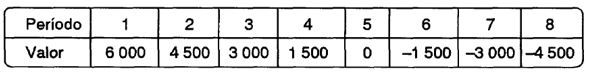
\includegraphics[height = 2.0cm]{E6_3}
       \end{center}
       \textbf{Respuesta:} COP 17.077\\
       \medskip

 \item 4. Hallar el valor de  COP  "R" del siguiente flujo de caja, con intereses al 30\% "nominal anual año vencido"\\.
       \begin{center}
        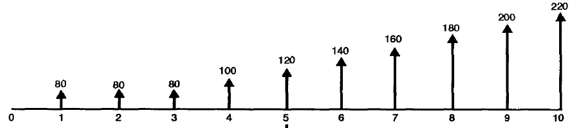
\includegraphics[height = 3.0cm]{E6_4}
       \end{center}
       \textbf{Respuesta:} COP 1 203,02\\
       \medskip

 \item 5. Hallar el valor de  COP  "R" del siguiente flujo de caja, con tasa del 20\% "nominal anual año vencido".
       \begin{center}
        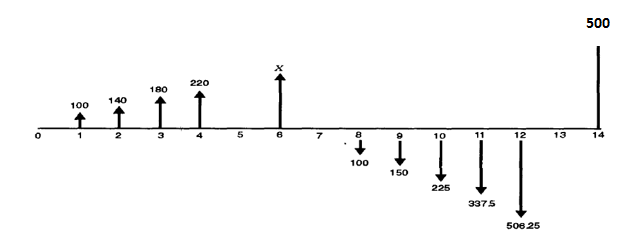
\includegraphics[height = 5.5cm]{E6_5}
       \end{center}
       \textbf{Respuesta:} COP 713.33. Significa que R tiene sentido opuesto al que aparece en la gráfica.\\
       \medskip

 \item 6. Con tasa del 25\% "nominal anual año vencido", hallar  COP  "R" del siguiente flujo de caja.
       \begin{center}
        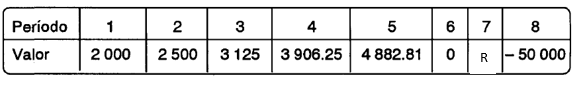
\includegraphics[height = 2.0cm]{E6_6}
       \end{center}
       \textbf{Respuesta:} COP 1 853.03\\
       \medskip

 \item 7. Hallar el primer pago de un gradiente lineal creciente en COP 300.000, que tenga 50 pagos anuales y que sea equivalente a 50 pagos anuales que crecen un 20\%, con primer pago de COP 1'000.000, suponga una tasa del 20\% "nominal anual año vencido"\\.
       \medskip

 \item 8. Una persona quiere comprar un automóvil, que actualmente cuesta COP 4 millones; para tal fin, decide establecer un fondo mediante depósitos mensuales crecientes en un 4\%. Si el primer depósito es de COP 60.000, que se hace al final de un mes, ¿cuánto tiempo le llevará reunir el dinero necesario para la compra, si el automóvil sube de precio cada mes un 1\%? Suponga una tasa del 4\% periódico mensual vencido.\\
       \textbf{Sugerencia:} Calcule el tiempo por interpolación.\\
       \textbf{Respuesta:} 29.35 meses, luego debe esperar 30 meses.\\
       \medskip

 \item 9. ¿Cuántos pagos mensuales deben hacerse para cancelar una deuda de COP 2 millones, con intereses del 36\% nominal anual mes vencido, suponga que la primera cuota es de COP 50.000 y que la cuota crece en COP 500 mensualmente.\\
       \textbf{Respuesta:} Por interpolación 96.29 períodos, luego debe esperar 97 períodos.\\
       \medskip

 \item 10. Con interés efectivo del 14 \% "nominal anual año vencido", hallar el valor final de la siguiente serie:\\
       \begin{center}
        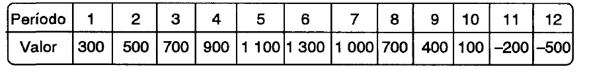
\includegraphics[height = 2.0cm]{E6_10}
       \end{center}
       \textbf{Respuesta:} COP 16673.39\\
       \medskip

 \item 11. Con interés efectivo del 10\% "nominal anual año vencido" hallar el valor presente de la siguiente serie utilizando gradientes:
       \begin{center}
        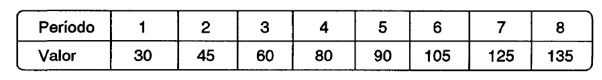
\includegraphics[height = 2.0cm]{E6_11}
       \end{center}
       \textbf{Sugerencia:} divida las cuotas de los períodos 4 y 7, de forma tal que una parte esté de acuerdo con la ley de formación del gradiente y el excedente lo puede considerar como cuota adicional.\\
       \textbf{Respuesta:} COP 406.46\
       \medskip

 \item 12. Con interés efectivo del 10\% "nominal anual año vencido", hallar el valor presente de la siguiente serie utilizando gradientes:\\
       \begin{center}
        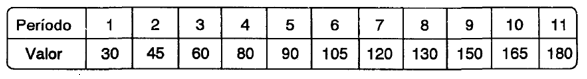
\includegraphics[height = 2.0cm]{E6_12}
       \end{center}
       \textbf{Respuesta:} COP 591.87\\
       \medskip

 \item 13. Con una tasa del 6\% "nominal anual año vencido" hallar el valor presente de la siguiente serie usando gradiente.\\
       \begin{center}
        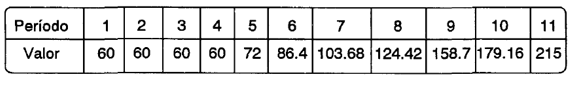
\includegraphics[height = 2.0cm]{E6_13}
       \end{center}
       \textbf{Respuesta:} COP 776.86\\
       \medskip

 \item 14. Hallar el valor presente de una serie infinita de pagos si el primero vale COP 100.000 y son crecientes en un 10\%. Suponga una tasa efectiva del 8\% "nominal anual año vencido"\\.
       \medskip

 \item 15. ¿Cuál es el valor presente de una serie infinita de pagos mensuales que crecen cada mes en COP 300.000 y cuyo primer pago es de COP 200.000. Suponga una tasa del 2.5\% período mes vencido.\\
       \medskip

 \item 16. Para mantener en buen estado una carretera veredal, los hacendados de la región desean establecer un fondo, para proveer las reparaciones futuras. Estas se estiman en un millón de pesos para el próximo año; también, se estima que su costo se incrementará todos los años en un 18\%. Hallar el valor del fondo, suponiendo un interés del 28\% "nominal anual año vencido"\\.
       \textbf{Respuesta:} COP 10.000 000\\
       \medskip

 \item 17.Hallar el valor presente de 24 pagos mensuales que crecen cada mes un 2\%. Suponga una tasa del 2\% período mes vencido y que el primer pago es de COP 500.000.\\
       \medskip

 \item 18.Hallar el valor presente de un gradiente infinito de pagos mensuales que crecen un 2\% y cuyo primer pago es de COP 800.000\\.
       a. Suponga una tasa del 3\% período mes vencido.\\
       b Suponga una tasa del 1,5\% período mes vencido.\\
       \medskip

 \item 19.¿A qué tasa anual efectiva se cumplen las condiciones mostradas en el siguiente diagrama?\\
       \begin{center}
        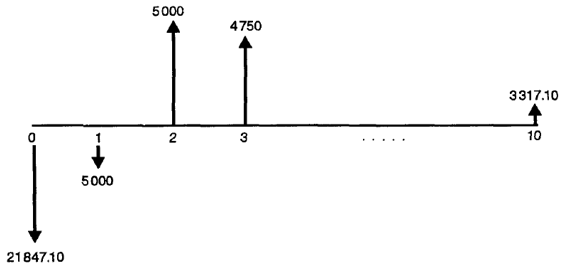
\includegraphics[height = 5.0cm]{E6_19}
       \end{center}
       \textbf{Respuesta:} 6.25\% "nominal anual año vencido"\\
       \medskip

 \item 20. ¿A qué tasa efectiva se cumplen las condiciones mostradas en el siguiente diagrama?\\
       \begin{center}
        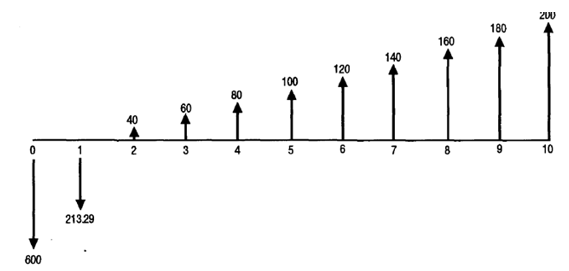
\includegraphics[height = 5.3cm]{E6_20}
       \end{center}
       \textbf{Respuesta:} 4,3\% "nominal anual año vencido"\\
       \medskip

 \item 21. Reemplazar el siguiente flujo de caja, por una serie uniforme, de igual número de pagos anuales, con una tasa del 20\% "nominal anual año vencido".\\
       \begin{center}
        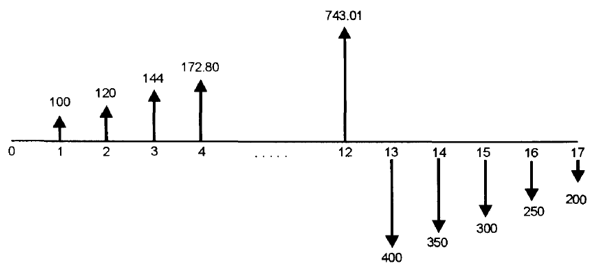
\includegraphics[height = 5.3cm]{E6_21}
       \end{center}
       \textbf{Respuesta:} 187,10\%\\
       \medskip

 \item 22. Un padre desea reunir una cantidad mediante depósitos anuales uniformes, comenzando hoy (primero de enero de 1984) y terminando el primero de enero de 1990, en un fondo que paga el 28\% nominal anual semestre vencido, su objetivo es el de garantizar a su hijo el estudio universitario, que se estima durará unos 6 años y empezará el primero de enero de 2015. Actualmente, la matrícula semestral cuesta COP 300.000, pero aumentará todos los semestres un 8\%. Calcular el valor de los depósitos anuales.\\
       \textbf{Sugerencia:} calcular el valor de la matrícula el primero de enero de 1990.\\
       \medskip

 \item 23. Una entidad financiera presta a un cliente COP 3 millones, con un interés del 34.8\% nominal anual mes vencido. El deudor tiene un plazo de 15 años para amortizar la deuda, mediante pagos mensuales. Suponiendo que la primera cuota es de COP 100.000 y vence al final del primer mes, ¿cuál debe ser el porcentaje de reajuste mensual de la cuota, para cancelar la deuda?\\
       \medskip

 \item 24. [verificar] Se ofrece la administración de un restaurante durante un año y se garantiza que comprarán exactamente 6000 almuerzos mensuales durante ese año, los cuales serán pagaderos en un solo contado a razón de COP 500 cada uno, pero su valor total será cancelado al final del año sin intereses, la persona calcula que el costo de los insumos de cada almuerzo será de COP 200 los cuales deberán ser adquiridos y pagados al principio de cada mes y su valor aumentará cada mes un 5\%. El costo mensual de mano de obra se considera estable en COP 250.000 y además, se requerirá una inversión inicial de COP 1 millón para la adecuación del restaurante. Suponiendo un interés mensual del 3\% período mes vencido. Calcular cuál será el valor de su ganancia:\\
       a.en pesos de hoy.\\
       b. en pesos futuros.\\
       \textbf{Respuestas:} a. COP 5.719.285 \hspace{1cm}  	b. COP 8.154.333\\
       \medskip

 \item 25. Resuelva el problema anterior suponiendo que en el mes 6 debe pagar a sus empleados, además de su sueldo, una bonificación de COP 125000 y en el mes 12 deberá pagar adicionalmente COP 400000 por prestaciones sociales.\\
       \textbf{Respuestas:}  a. COP 5.334.048 \hspace{1cm}  	b. COP 7.605.077\\
       \medskip

 \item 26. Resuelva el problema 24 suponiendo que el valor de los almuerzos sea pagadero al final de cada mes.
       \textbf{Respuestas:} a. COP 10.331.622 \hspace{1cm}  	b. COP 14.730.422\\
       \medskip

 \item 27. Una fábrica tiene costos fijos de COP 600.000 mensuales y costos variables de COP 150 por unidad. Durante los primeros 6 meses no hay producción porque este tiempo se dedicará a pruebas y ajustes. En el mes 7 se iniciará la producción con 300 unidades y cada mes la producción aumentará en 200 unidades hasta llegar al tope de 2.500 al mes. Si se espera vender la fábrica al final de 3 años, calcular el costo total de la producción en estos 3 años en pesos de hoy. Suponga una tasa del 3\% periódico  mensual vencido.\\
       \textbf{Respuesta:}  COP 17.791.600\\
       \medskip

 \item 28. Una máquina produce una utilidad de un millón de pesos durante el primer año, sin embargo, la utilidad de la máquina disminuye COP 350.000 cada año debido al desgaste. Calcular en pesos de hoy el total de las ganancias suponiendo que la máquina va a trabajar por 10 años. Utilice una tasa del 30\% "nominal anual año vencido".\\
       \medskip

 \item 29. Una fábrica debe importar 80 toneladas mensuales de materia prima pagándola al principio de cada mes en dólares de Estados Unidos a razón de USD200 la tonelada. Según la experiencia se observa que el peso se devalúa a razón del 2.5\% mensual con relación al dólar. Si el cambio actual es de USD1 = COP 4.000 hallar el valor total de las importaciones de la fábrica en el transcurso de un año\\.
       a. En pesos de principio de año.\\
       b. En pesos de final del año. Suponga que la fábrica trabaja con una tasa del 3\% periódico  mensual vencido.\\
       \medskip

 \item 30. Resuelva el problema anterior suponiendo que el fabricante efectúa las importaciones mediante cartas de crédito las cuales deberá cancelar a los 2 meses de su emisión.\\
       \textbf{Respuestas:} a. COP 74.058.054 \hspace{1,0cm}  b. COP 105.589.077\\
       \medskip

 \item 31. Una empresa está preparando su plan quinquenal de gastos. La nómina mensual actual vale COP 2 millones y se estima que cada año el salario mensual se incrementará en un 25\%. ¿Cuál debe ser el valor de la provisión en pesos de hoy para el presente quinquenio? suponga que la empresa utiliza una tasa de interés del 35\% "nominal anual año vencido".\\
       \textbf{Respuesta:} COP 88292.236\\
       \medskip

 \item 32.El banco ABC concede un préstamo para adquirir un local comercial por COP 5 millones el día primero de octubre de 1992, en las siguientes condiciones: plazo 12 años, pagos mensuales crecientes en un 1\% y tasa del 36\% nominal anual mes vencido. El día primero de agosto de 1999 el deudor solicita al banco XYZ la refinanciación de la deuda que en ese momento tiene contraída con el banco ABC. El nuevo préstamo se efectúa en las siguientes condiciones: cuotas mensuales crecientes en un 1.2\%, tasa 30\% nominal anual mes vencido, plazo 15 años. ¿Cuál será el valor de la cuota que el primero de septiembre de 1999 pagaría al banco ABC en caso de no haber refinanciación? y ¿Cuál sería el valor de la cuota que en esa misma fecha pagarla al banco XYZ en caso de refinanciación?\\
       \textbf{Respuesta:} Cuota en ABC = COP 240.404.90, \hspace{1,0cm} Cuota en XYZ = COP 122.215.46.\\

\end{itemize}

\chapter*{Capítulo 7}
\addcontentsline{toc}{chapter}{\textcolor{ocre}{Capítulo 7}}




\begin{itemize}
 \item 1)	Elaborar una tabla para amortizar la suma de COP 3'000.000 en 4 pagos trimestrales uniformes con una cuota extraordinaria de COP 500.000 en el período 3, suponga una tasa del 10\% efectiva anual para el período. \\
       \medskip

 \item 2)	Un automóvil cuesta COP 4.000.000, se puede financiar al 60\% para ser pagado en cuotas mensuales durante 3 años con un interés del 36\% nominal anual mes vencido: Hallar la cuota mensual.\\
       \textbf{ Respuesta:} COP 109.929.11
       \medskip

 \item 3)	Si en el problema anterior se ofrecen cuotas extraordinarias cada 6 meses del doble de la cuota ordinaria. ¿Cuál sería el valor de la cuota ordinaria?\\
       Sugerencia: observe que hay dos series uniformes, una simple y otra del tipo general.\\
       \textbf{Respuesta:} COP 83.966.95
       \medskip

 \item 4)	Elaborar una tabla para amortizar COP 800.000 en 5 pagos semestrales mediante el sistema de abono constante a capital y con una tasa del 30\% nasa (nominal anual semestre anticipado).
       \medskip

 \item 5)	 Hallar el valor de la cuota de amortización de una deuda de COP 1.000.000 la cual va a ser cancelada en las siguientes condiciones:\\
       a.	número de pagos ordinarios 4;\\
       b.	número de períodos de gracia muertos 2\\
       c.	tasa 10\% efectiva anual para el período \\
       d.	elabore la tabla de amortización\\
       \textbf{ Respuesta:} COP 381.719.70
       \medskip

 \item 6)	Resolver el problema anterior suponiendo que el plazo de gracia es de cuota reducida (plazo en el que solo se pagan los intereses). Elabore la tabla de amortización.\\
       \textbf{Respuesta: }COP 315.470.80
       \medskip

 \item 7)	Elaborar una tabla para amortizar la suma de COP 300.000, bajo las siguientes condiciones:\\
       a.	número de pagos ordinarios: 5;\\
       b.	plazo de gracia muerto: 1 período;\\
       c.	cuotas extraordinarias: 2; la primera de COP 35.000, en el período 3 y la segunda de COP 50.000 en el período 5;\\
       d.	tasa 8\% efectiva anual para el período.\\
       \textbf{Respuesta:} COP 64.427.83
       \medskip

 \item 8)	El día primero de abril de 1986, se contrae una deuda de COP 200.000, para ser pagada en cuotas trimestrales ordinarias; la primera se efectuará el primero de octubre de 1986 y la última el primero de julio de 1987, más una cuota extraordinaria de COP 50.000, el primero de enero de 1987. Suponiendo una tasa del 36\% nominal anual año vencido, elaborar la tabla de amortización.\\
       \textbf{Respuesta parcial:} valor de la cuota ordinaria COP 54.299.76
       \medskip

 \item 9)	Una deuda de COP 1 millón viene siendo amortizada en pagos trimestrales durante 2 años, con un interés del 42\% nominal anual año vencido . Inmediatamente después de efectuar el tercer pago trimestral el deudor hace un abono extraordinario no pactado de COP 300.000 y solicita que le presenten un plan de amortización tomando en cuenta dos alternativas, la primera, abonar a capital acortando el tiempo y manteniendo inalteradas las cuotas trimestrales y la segunda, abonar a capital y re-liquidar la cuota dejando inalterado el número total de pagos. Elabore una tabla para la amortización del saldo en cada caso.\\
       \textbf{Respuesta:}\\
       Primera alternativa
       \begin{center}
        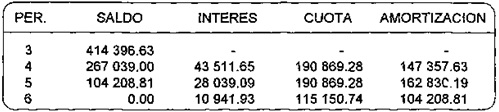
\includegraphics[height=3.0cm]{E7_9_1}
       \end{center}
       Segunda alternativa:
       \begin{center}
        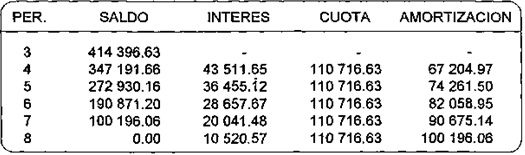
\includegraphics[height=4.0cm]{E7_9_2}
       \end{center}
       \medskip

 \item 10)	 Elaborar una tabla de capitalización para reunir la suma de COP3'500.000 en cuatro depósitos ordinarios de  COP  "R" c/u, más un depósito extraordinario de COP600.000, que se hará conjuntamente con el tercer depósito ordinario. Suponga una tasa del 9\% "nominal anual año vencido" para el período.\\
       \medskip

 \item 11)	 Elaborar una tabla, para que el día primero de septiembre de 1988 se hayan reunido COP500.000 en las siguientes condiciones:\\
       a.	depósitos semestrales ordinarios de  COP  "R" c/u; el primer depósito se efectuará el primero de marzo de 1986; el último depósito se efectuará el primero de septiembre de 1987; \\
       b.	se hará un depósito extraordinario de COP70.000 el primero de marzo de 1987;\\
       c.	tasa 30\% nominal anual semestre vencido.\\
       \textbf{Respuesta:}
       \begin{center}
        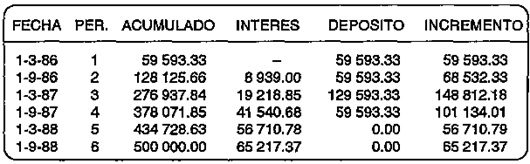
\includegraphics[height=4.0cm]{E7_11}
       \end{center}
       \medskip

 \item 12)	 Una deuda de COP 2 millones está siendo amortizada mediante pagos mensuales uniformes, durante 15 años, con un interés del 27.6\% nominal anual mes vencido. Determinar qué parte del pago número 64 se utiliza a pagar intereses y cuánto a amortización.\\
       \textbf{ Respuesta:} intereses COP 43.510.12; amortización, COP 3.270.52
       \medskip

 \item 13)	 Se están reuniendo COP 2 millones, mediante depósitos mensuales uniformes durante 5 años, en un fondo que paga el 30\% nominal anual mes vencido. Determinar cuál es el crecimiento del fondo, por concepto de intereses en el período 41. \\
       \textbf{Respuesta:} COP 24.781.88
       \medskip

 \item 14)	 Una deuda de COP 1.000 000 está siendo amortizada en pagos mensuales durante 15 años, con intereses al 30\% nominal anual mes vencido. Elaborar una tabla de amortización que muestre, únicamente, los períodos 108,109 y 110.\\
       \textbf{Respuesta:}
       \begin{center}
        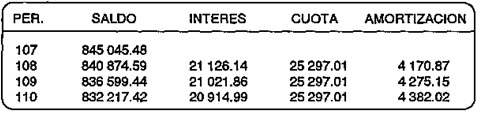
\includegraphics[height=3.5cm]{E7_14}
       \end{center}
       \medskip

 \item 15)	 Se está reuniendo un capital de COP 1.000.000, mediante depósitos mensuales iguales durante 8 años en un fondo que paga el 30\% nominal anual mes vencido. Además, se ha acordado que, al momento de efectuar el depósito ordinario número 56, se hará un depósito extraordinario de COP 70.000. Construir una tabla que muestre, únicamente los períodos 55, 56 y 57.\\
       \textbf{Respuesta:}
       \begin{center}
        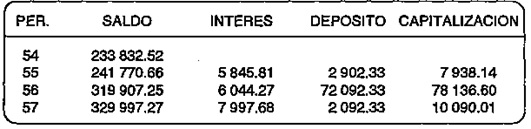
\includegraphics[height=4.0cm]{E7_15}
       \end{center}
       \medskip

 \item 16)	 Elaborar una tabla para amortizar la suma de COP 600.000 en 6 pagos trimestrales, con cobro anticipado de intereses del 8.5\% ptv periodo trimestre vencido y abonos vencidos e iguales a capital.
       \medskip

 \item 17)   Hallar el valor de la cuota total (intereses + amortización) que debe pagarse al final del mes 20 en una amortización de COP 3 millones en pagos mensuales, durante 3 años, con cobro anticipado de intereses y abono a capital mensuales e iguales. Suponga una tasa del 2.5\% período mes anticipado.\\
       \textbf{Respuesta: }COP 116 666.73
       \medskip

 \item 18)	 Hallar la primera cuota de amortización necesaria, para cancelar una deuda de COP 100.000 en las siguientes condiciones:\\
       a. plazo de gracia muerto: 2 períodos; \\
       b. número de cuotas ordinarias: 4; \\
       c. cuota extraordinaria pactada de COP 20.000, en el período 4 (coincide con el segundo pago ordinario); \\
       d. tasa 10\% anual efectiva para el período; \\
       e. característica de la cuota ordinaria:\\
       $e_{1}$)  Creciente lineal en COP 6.000 \\
       $e_{2}$)  Decreciente lineal en -COP 6.000\\
       \textbf{Respuestas:} $e_{1}$)  COP 24 670.57;  $e_{2}$)  COP 41 244.58
       \medskip

 \item 19) Hallar la primera cuota de amortización necesaria, para cancelar una deuda de COP 100.000 en las siguientes condiciones:\\
       a.	plazo de gracia muerto: 2 períodos; \\
       b.	número de cuotas ordinarias: 4;\\
       c.	cuota extraordinaria pactada de COP 20 000, en el período 4 (coincide con el segundo pago ordinario); \\
       d.	tasa 10\% anual efectiva para el período; \\
       e.	característica de la cuota ordinaria:\\
       $e_{1}$)  Creciente geométrica en 20\%\\
       $e_{2}$)  Decreciente geométrico en - 20\%\\
       \textbf{Respuestas: }$e_{1}$)  COP 41 244.58;  $e_{2}$)  COP 25 095.34\\
       \medskip

 \item 20)	 Elaborar una tabla en períodos anuales, que muestre la amortización de COP 300.000 en 4 pagos, pero cada pago se efectúa cada 2 años y son crecientes en un 30\%. Suponga una tasa del 24\% "nominal anual año vencido".\\
       \textbf{Respuesta}
       \begin{center}
        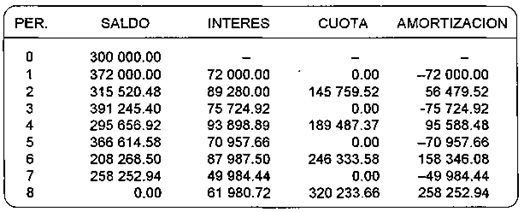
\includegraphics[height=4.0cm]{E7_20}
       \end{center}
       \medskip

 \item 21)  Elaborar una tabla de amortización para cancelar una deuda de COP 700.000 en 3 años mediante pagos semestrales bajo las siguientes condiciones: tasa de interés 28\% nominal anual semestre vencido. dentro de cada año, el pago permanece constante pero; cada año:\\
       a.	el valor del pago aumenta un 20\% \\
       b.	el valor del pago disminuye un 20\% \\
       \textbf{Respuestas:}
       a)
       \begin{center}
        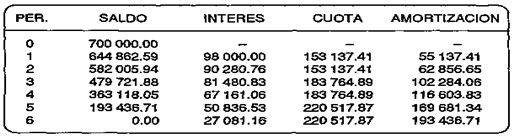
\includegraphics[height=4.0cm]{E7_21_1}
       \end{center}
       b)
       \begin{center}
        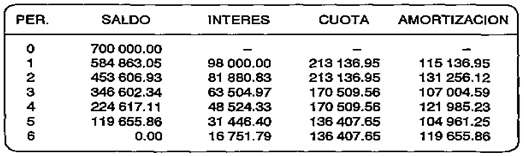
\includegraphics[height=4.0cm]{E7_21_2}
       \end{center}
       \medskip

 \item 22) Resuelva el problema anterior suponiendo que:\\

       a)	el pago global anual aumenta en COP 15.000 (esto equivale a decir que: el valor de los pagos del gradiente aumentan en COP 15.000 pero la diferencia entre las inter-cuotas no es de COP 15.000) \\
       b)	el pago global anual disminuye en COP 15.000\\
       \textbf{ Respuestas:}
       a)
       \begin{center}
        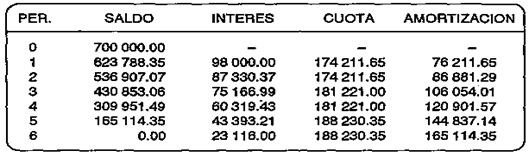
\includegraphics[height=4.0cm]{E7_22_1}
       \end{center}
       b)
       \begin{center}
        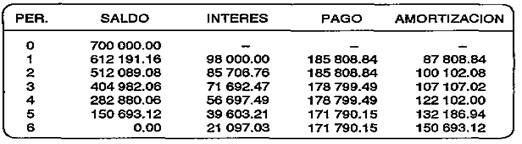
\includegraphics[height=4.0cm]{E7_22_2}
       \end{center}
       \medskip

 \item 23) Elaborar una tabla para amortizar la suma de COP 900.000 en pagos semestrales durante 3 años, con la condición de aumentar cada año el valor de los pagos en COP 60.000 pero dentro de cada año el valor de los pagos permanecen constantes. Utilice una tasa del 38\% nominal anual semestre vencido.\\
       \textbf{Respuesta:}\\
       \begin{center}
        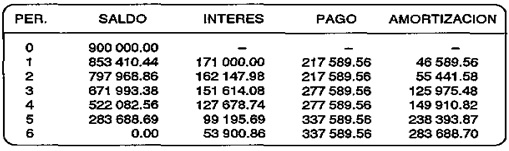
\includegraphics[height=4.0cm]{E7_23}
       \end{center}
       \medskip

 \item 24)	 Elaborar una tabla para amortizar la suma de COP 800.000 en pagos semestrales durante 3 años, pero que crecen cada año en COP 50.000, con una tasa del 42\% nominal anual semestre vencido.\\
       \textbf{Respuesta:}
       \begin{center}
        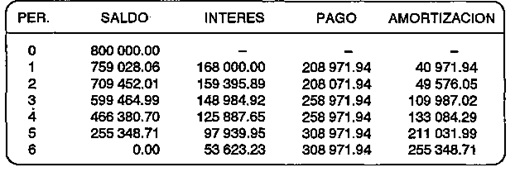
\includegraphics[height=4.0cm]{E7_24}
       \end{center}
       \medskip

 \item 25)	 Elaborar una tabla para amortizar la suma de COP 100.000 en dos años, más un período de gracia muerto de 6 meses, con intereses al 30\% nominal anual mes vencido, mediante pagos trimestrales iguales, pero con crecimiento anual de la cuota del 21\% (escalonado). Además, se efectuará un pago extraordinario de COP 20.000, al final del mes 18.\\
       \textbf{Respuesta:}
       \begin{center}
        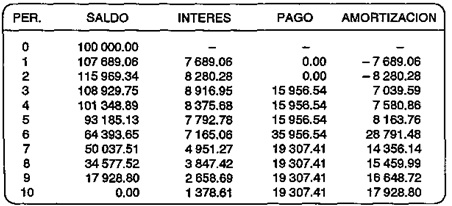
\includegraphics[height=4.0cm]{E7_25}
       \end{center}
       \medskip

 \item 26)	 Elaborar una tabla para capitalizar COP 200.000 en 3 años, más un período de gracia de un año, mediante depósitos semestrales ordinarios que crezcan cada año un 25\%, pero el valor de los depósitos es constante; además se efectuará un depósito extraordinario de COP 40.000 en el período 3. Suponga un interés del 32\% nominal anual semestre vencido.\\
       \textbf{Respuesta:}
       \begin{center}
        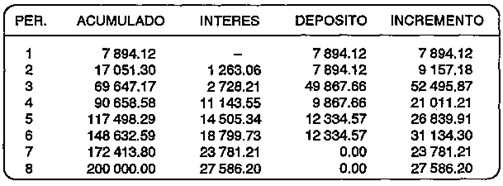
\includegraphics[height=4.0cm]{E7_26}
       \end{center}
       \medskip

 \item 27)	 Desea amortizarse la suma de COP 5 millones, en cuotas mensuales, durante 20 años, con la condición de aumentar cada cuatro años la cuota mensual en un 50\%. Si suponemos una tasa del 32\% "nominal anual año vencido", calcular el valor del primero y del último pago. \\
       \textbf{Respuestas:} COP 90.966.36 y COP 460.517.19
       \medskip

 \item 28)	 Una deuda de COP 2 millones está siendo amortizada en pagos mensuales, durante 15 años, con intereses al 30\% nominal anual mes vencido y crecimiento mensual de la cuota de COP 300. Hallar la distribución del pago 105, entre intereses y abono a capital.\\
       \textbf{Respuesta:} intereses: COP 66.323.59; amortización: COP 4.111.98
       \medskip

 \item 29)	 Se está reuniendo la suma de COP 5 millones mediante depósitos mensuales durante 8 años. Si los depósitos aumentan de valor cada mes COP 200 y suponiendo un interés del 27\% nominal anual mes vencido:\\
       a.	calcular el capital reunido hasta el período 63 \\
       b.	¿qué tanto del incremento al fondo en el período 64 es debido a intereses? \\
       \textbf{Respuestas: }a) COP 1.840.961.97;  b) COP 41.421.64
       \medskip

 \item 30)	 Una persona se compromete a cancelar una deuda de COP 400.000, con intereses al 36\% nominal anual año vencido, mediante pagos trimestrales durante 10 años. Cada año, el valor de las cuotas crece un 15\%, pero dentro de cada año la cuota no varía. Determinar el valor de la cuota número 14, su distribución entre intereses y abono a capital y el saldo insoluto, inmediatamente después de haberse efectuado el pago número 14.\\
       \textbf{Respuestas:} valor de la cuota: COP 39 942; 	intereses: COP 48 590.21;
       Amortización: -COP 8 648.22;       saldo: COP 548 539.49\\
       \medskip

 \item 31)	 Una deuda de COP 2 millones está siendo amortizada en pagos mensuales, durante 15 años, con la condición de incrementar la cuota cada año en un 18\% pero dentro de cada año la cuota permanece constante. Suponiendo un interés del 27\% nominal anual mes vencido, determinar:\\
       a.	el valor del primer pago; \\
       b.	el valor del último pago; \\
       c.	 la deuda, inmediatamente después de haber efectuado el pago 1 00; \\
       d.	la distribución del pago 101. \\
       \textbf{Respuestas: }a) COP 23 706.16;	 b) COP 240 552.22; 	e) COP 4 976 930.72;
       d. interés: COP 111 980.94, amortización: - COP 22 872.81
       \medskip

 \item 32)	 Elaborar una tabla para amortizar la suma de COP 700.000, en pagos semestrales, con las siguientes condiciones:\\
       a.	el primer año se otorga, como período de gracia muerto (significa que no hay pagos y los intereses que se causan se abonan a capital)\\
       b.	el segundo año se otorga como período de gracia con cuota reducida( significa que solo, se pagan intereses pero no hay abono a capital) \\
       c.	en los siguientes 2 años se efectuarán pagos semestrales ordinarios crecientes en un 15\% \\
       d.	debe incluirse una cuota extra de COP 50.000 en el período 6 (la cuota extra coincide con el segundo pago ordinario) \\
       e.	tasa de interés: 30\% nominal anual semestre vencido.\\

       \textbf{ Respuesta:}
       \begin{center}
        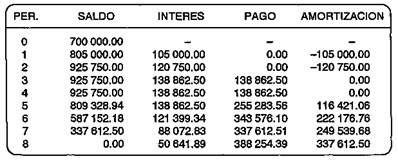
\includegraphics[height=4.0cm]{E7_32}
       \end{center}
       \medskip

 \item 33)	 Resolver el problema anterior, suponiendo que el crecimiento es escalonado anual del 15\%. \\
       \textbf{Respuesta:}
       \begin{center}
        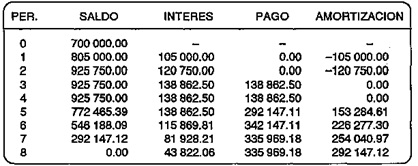
\includegraphics[height=4.0cm]{E7_33}
       \end{center}
       \medskip

 \item 34) Elaborar una tabla para amortizar la suma de COP 800.000, en valor constante, mediante pagos trimestrales, durante 15 meses, suponiendo un interés del 30\% nominal anual año vencido y que el índice de corrección monetaria permanecerá constante en el 8\% período mes vencido .\\
       \textbf{ Respuesta:}
       \begin{center}
        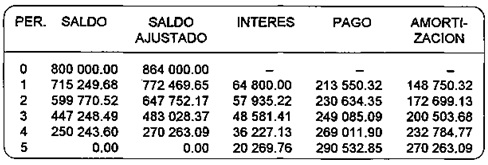
\includegraphics[height=4.0cm]{E7_34}
       \end{center}
       \medskip

 \item 35)   Elaborar una tabla para amortizar la suma de COP 600.000, en cuatro pagos trimestrales decrecientes en COP 50.000; pero en valor constante, utilice un interés del 8\% nominal anual año vencido y suponga que la tasa de corrección monetaria permanecerá constante en el 22\% nominal anual año vencido.
       \textbf{Respuesta:}
       \begin{center}
        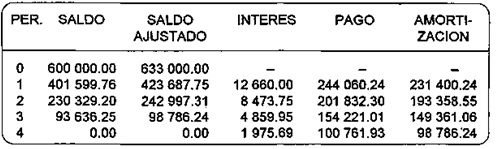
\includegraphics[height=4.0cm]{E7_35}
       \end{center}
       \medskip

 \item 36) Elaborar una tabla para amortizar en valor constante la suma de COP 600.000, en 3 pagos anuales que decrecen anualmente en un 20\%. Suponga que la corrección monetaria permanece constante en el 22\% "nominal anual año vencido" y que se cobra un interés del 10\% "nominal anual año vencido". \\
       \textbf{Respuesta}
       \begin{center}
        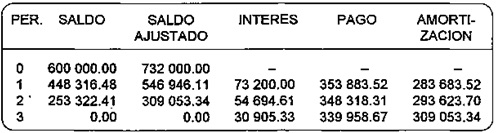
\includegraphics[height=4.0cm]{E7_36}
       \end{center}
       \medskip

 \item  37) Suponga que en el problema anterior el gradiente es escalonado, con pagos semestrales.\\

       \textbf{ Respuesta:}
       \begin{center}
        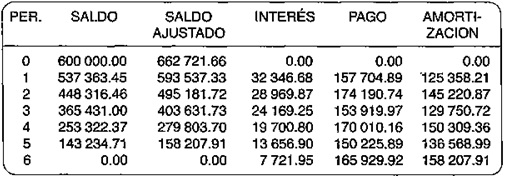
\includegraphics[height=4.0cm]{E7_37}
       \end{center}
       \medskip

 \item 38)  Un préstamo por valor de COP 3 millones a 15 años con una tasa del 2.75\% período mes vencido  va ser amortizado en pagos mensuales durante 15 años con la condición de aumentar anualmente la cuota mensual en un 18\% durante los primeros 8 años y de ahí en adelante las cuotas mensuales crecerán anualmente en un 12\%. Calcular el valor de las cuotas durante el primer año y el valor da las cuotas durante el noveno año. \\
       \textbf{Respuestas:} cuota mensual primer año COP 49 900.69;
       Cuota mensual noveno año COP 178 032.24
       \medskip

 \item 39)  Elaborar una tabla para amortizar la suma de COP 12 millones si el crédito es concedido por una entidad financiera que cobra la tasa Libor + 8 puntos, para ser pagado en cuatro cuotas trimestrales vencidas en dólares. Al momento de otorgar el crédito se conoce la siguiente información: \\
       a.	Cambio USCOP 1 = COP 3.000 \\
       b.	Tasa de devaluación proyectada 7\% "nominal anual año vencido", se asume que la devaluación es uniforme a través del año. \\
       c.	Tasa Libor = 2\% "nominal anual año vencido", se presume que no va a variar. \\

       Elabore una tabla que como mínimo muestre, en pesos, el saldo y el pago. Trabajar cualquier tasa con 5 decimales.\\
       Recuerde que cuando sume dos tasas efectivas debe usar la tasa    combinada.\\

       \textbf{ Respuesta:}
       \begin{center}
        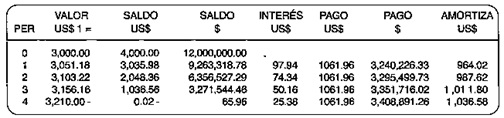
\includegraphics[height=4.0cm]{E7_39}
       \end{center}
       \medskip

 \item 40)  Elaborar una tabla para amortizar la suma de COP 3 millones a la tasa del 18\% nominal anual semestre vencido a un plazo de 3 años con cuotas semestrales por el sistema de abonos pactados a capital.\\
       
      Se ha pactado que en cada uno de los semestres 1 y 2 se amortiza el 1 0\% de la deuda.\\
       En cada uno de los semestres 3 y 4 se amortiza el 20\% de la deuda. \\
       En cada uno de los semestres 5 y 6 se amortiza el 25\% de la deuda.\\
       \textbf{Respuesta parcial:} el valor de los pagos será: COP 270.000, 243.000, 216.000, 175.500, 135.000, 67.500
       \medskip

 \item 41)  Elaborar una tabla para amortizar la suma de COP 4 millones en pagos trimestrales durante un año por el sistema de cuota fija con tasa variable. Tasa de interés DTF + 14 puntos. \\

       En el momento de otorgar el crédito la DTF = 7.5\% NTA.\\

       A los 3 meses la DTF = 7.7\% NTA\\
       A los 6 meses la DTF = 7.9\% NTA \\
       A los 3 meses la DTF = 8.3\% NTA \\
       A los 3 meses la DTF = 7.8\% NTA\\
       Trabajar las tasa con 5 decimales\\
       \textbf{Respuesta parcial:} Cuota fija COP 1.145.927.48, valor del último pago COP 1 158.346.26.
       \medskip

 \item 42)  Una empresa necesita cambiar de vehículo cada 3 años dando en parte de pago el vehículo usado y el resto se cancelará al contado con dineros provenientes de un fondo que paga el 33\% nominal anual mes vencido. Calcular el valor del depósito mensual uniforme necesario suponiendo las siguientes condiciones: \\

       a.	el precio actual, del vehículo nuevo es de COP 6 millones y cada 3 meses aumenta de precio un 4.8\%.
       b.	el vehículo, que se compre actualmente, a pesar de su uso y debido a procesos inflacionarios sube de precio cada 3 meses a razón del 3.2\%.\\
       \textbf{Respuesta:} COP 29.491.33
       \medskip

 \item 43) Suponga que en el ejemplo anterior el fondo paga el 32\% nominal anual año vencido y se constituye mediante depósitos trimestrales crecientes en un 8\%. Hallar el depósito en el fondo del primero y del último trimestre.\\
       \textbf{Respuestas:} COP 63.452.34 y COP 147.947.94
       \medskip

 \item 44)  Actualmente se contrae una deuda de COP 600.000 para ser cancelada al final de 2 años y mientras tanto se deberá pagar un interés del 40\% nominal anual año vencido. A fin de dar cumplimiento al pago de la deuda en su debida oportunidad se constituye un fondo de amortización que paga el 36\% nominal anual año vencido mediante depósitos trimestrales iguales. \\

       a.	calcular el costo trimestral de la deuda.\\
       b.	si en lugar de constituir el fondo de amortización se hace una amortización usando como cuota de amortización el costo trimestral de la deuda. ¿A qué tasa nominal capitalizable trimestralmente se estaría amortizando la deuda?\\
       \textbf{Respuestas:} a) COP 114.404.13 b) 41.89\%  nominal anual año vencido.
       \medskip

 \item 45) En el problema anterior. ¿Qué tanto del incremento al fondo en el período 7 es debido a intereses? \\
       \textbf{Respuesta:}COP 36.837.38
       \medskip

 \item 46) Elabore una tabla para el fondo.
       \medskip

 \item 47) Una persona deposita COP 1'000.000 en un fondo de amortización que paga el 21\% nominal anual mes vencido. Un año después comenzó a depositar en la misma cuenta COP 200.000 mensuales. ¿Cuánto tiempo tendrá que esperar para completar como mínimo COP 20.000.000? \\
       \medskip

 \item 48) Una persona depositó COP 100.000 trimestrales en un fondo de capitalización que pagaba el 28\% nominal anual año vencido.  Estos depósitos los hizo durante 5 años. A partir de ahí comenzó a retirar por semestre vencido la suma de COP 500.000. ¿Durante cuánto tiempo podrá retirar? \\
       \medskip

 \item 49) Usted desea capitalizar COP 10 millones. Para eso abre una cuenta hoy con COP 100.000 en un fondo de capitalización que paga el 2\% período mes vencido  y piensa depositar en esa cuenta COP 5.000 al final de cada mes. ¿Cuánto tiempo tendrá que estar haciendo estos abonos para que como mínimo alcance la meta que se propone? \\
       \textbf{Respuesta: }171 meses
       \medskip

 \item 50) Una deuda de COP 1.000.000 con intereses al 20\% nominal anual semestre vencido, se va a cancelar en pagos  durante 10 años. Inmediatamente después de efectuar el pago 12 deudor y acreedor acuerdan suspender los pagos semestrales y cancelar el saldo de la deuda de un solo contado a su vencimiento con sus respectivos intereses. Para dar cumplimiento al pago se constituye un fondo de amortización mediante depósitos mensuales iguales que ganan un interés del 2.8\% período mes vencido . \\

       a.	¿Cuáles son los derechos del deudor y acreedor inmediatamente después del pago 12? \\
       b.	¿Cuál debe ser el valor de los depósitos en el fondo?\\
       \textbf{Respuestas:} a) deudor COP 373.361.60; acreedor COP 626.638.40; b) COP 13.606.66

\end{itemize}


\chapter*{Capítulo 9}
\addcontentsline{toc}{chapter}{\textcolor{ocre}{Capítulo 1}}


\begin{itemize}
 \item 1. El ejecutivo de una fábrica propone adquirir una prensa, cuyo costo es de 52 millones; el dinero necesario puede ser adquirido mediante un préstamo del banco ABC, el cuál exige le sea cancelado en pagos mensuales uniformes, durante 3 años con un interés del 36\% CM. La prensa tiene una vida útil de 3 años y un valor de salvamento de COP 400 000, se espera que la prensa produzca ingresos mensuales por COP 83 000. Si el inversionista espera ganarse una tasa del 42\% CM. ¿Debe adquirirse la prensa? \\

       \textbf{Respuesta:} No se debe adquirir la prensa
       \medskip

 \item 2. Un industrial compró una máquina hace 3 años, en COP 600.000 y aun siguiendo las instrucciones del fabricante, su CAO se elevó a COP 220.000. Ahora un vendedor le ofrece otra máquina que está más de acuerdo con sus necesidades; esta nueva máquina cuesta COP 550.000 y le garantizan que su CAO no será superior a COP 100.000. Un avalúo que le hicieron a la máquina actual fue de COP 120.000 y por esta cantidad  hay oferta de compra, ¿será aconsejable el cambio, suponiendo una tasa del 28\%, que el valor de salvamento de ambas máquinas es prácticamente nulo y que se toma un horizonte de planeación de 10 años? \\

       \textbf{Respuesta:} No se aconseja cambiar de Maquina, -COP 876.891
       \medskip

 \item 3. Un laboratorio requiere un aislamiento térmico en paredes y cielo raso; para mantener una temperatura constante, se requiere el auxilio de calentadores y equipo de aire acondicionado. Existen en el mercado 3 tipos de aislamiento, que cumplen con las condiciones requeridas y, en todos los casos, prácticamente el valor de salvamento es nulo; además se conoce la siguiente información: \\

       \begin{table}[]
        \begin{tabular}{|l|l|l|l|l}
         \cline{1-4}
         Aislamiento                     & A( COP )   & B( COP )   & C( COP )   & \\ \cline{1-4}
         Costo Anual                     & 400.000 & 500.000 & 700.000 & \\ \cline{1-4}
         Costo Anual de Operacion        & 20.000  & 20.000  & 30.000  & \\ \cline{1-4}
         Vida Util                       & 4       & 5       & 30      & \\ \cline{1-4}
         Ahorro de energia al primer año & 100.000 & 200.000 & 300.000 & \\ \cline{1-4}
        \end{tabular}
       \end{table}

       La tarifa de energía sube anualmente un 8\%. Si se espera conservar el laboratorio por 10 años, ¿qué tipo de aislamiento debe utilizar? Suponga una tasa del 20\% efectiva anual.



       \textbf{Respuesta:} VPCc > VPNb > VPNa, Se debe seleccionar el aislamiento C COP 802.529,73 > COP 300.747,7054 > - COP 227.009,92
       \medskip

 \item 4. Una compañía está considerando la compra de una máquina manual que cuesta COP 30.000 y se espera que tenga una vida útil de 12 años, con un valor de salvamento de COP 3.000. Se espera que los costos anuales de operación sean de COP 9.000 durante los primeros 4 años pero que desciendan en COP 400 anuales durante los siguientes ocho años. La otra alternativa es comprar una máquina automatizada a un costo de COP 58.000. Esta máquina solo duraría 6 años a causa de su alta tecnología y diseño delicado. Su valor de salvamento será de COP 15.000. Por su automatización los costos de operación serán de COP 4.000 al año. Seleccionar la máquina usando una tasa del 20\%.\\

       \textbf{Respuesta:} Según los resultados arrojados se debe escoger la maquina manual. VPN=-COP 88.475.13008
       \begin{align*}
        VPN=-58.000-58.000\left(1+0,2\right)^{-6}-4.000\left[\frac{1-\left(1+0,2\right)^{-12}}{0,2}\right] \\ +15.000\left[\left(1+0,2\right)^{-6}+\left(1+0,2\right)^{-12}\right]
       \end{align*}
       \medskip

 \item 5. Determinar la mejor alternativa que tiene una fábrica para almacenar su materia prima y sus productos terminados, si ésta fábrica solo esperar trabajar 4 años; al final de los cuales entrará en liquidación. La Alternativa A consiste en comprar un terreno en COP 20.000.000 y construir una bodega, a un costo de COP 46.000.000; al final de los 4 años el terreno con la construcción podrán ser vendidos en COP 120.000.000. El CAO para el primer año, será de COP 200.000 y, cada año siguiente, se incrementará en un 15\%. La Alternativa B consiste en tomar en alquiler una bodega, a un costo de COP 10.000.000 por año anticipado y, cada año, el valor del arriendo sube un 20\%. Determinar la mejor alternativa, suponiendo que la tasa es del 20\%. \\

       \textbf{Alternativa A}
       \begin{align*}
        VPN=COP 120.000.000\left(1+0,2\right)^{-4}-COP 66.000.000-\left\{COP 200.000\left[\frac{\left(1+0,15\right)^4\left(1+0,2\right)^{-4}-1}{0,15-0,20}\right]\right\}
       \end{align*}
       VPN=-COP 8.755.774,981
       \\
       \textbf{Alternativa B}
       \begin{align*}
        VPN=\frac{-10.000.000\left(4\right)\left(1,2\right)}{1,2}=-COP 40.000.000
       \end{align*}
       \textbf{Respuesta:} Lo mas recomendable es elegir la alternativa A.
       \medskip

 \item 6. Para producir cierto artículo, una fábrica necesita hacer una inversión de COP 7.000.000 de los cuales COP 2.000.000 deberán ser financiados por un banco que le exige que se cancele el préstamo en 3 pagos anuales iguales, con intereses al 38\%. La capacidad máxima de la fábrica es de 20.000 unidades al año, pero el primer año solo estará en capacidad de producir el 40\%; el segundo año el 50\%, el tercer año el 75\%, el cuarto año el 90\% y el quinto año el 100\%. Cada artículo puede venderse en COP 2.000 durante el primero y el segundo año y en COP 2.400 del tercer año en adelante. Los costos de producción serán: materia prima COP 1.000 por unidad y cada año aumentara un 10\%; por sueldos, la nomina del primer año será de COP 2.500.000 y aumentara todos los años un 20\%. La maquinaria por valor de COP 5.000.000 será depreciada así: el primer año el 40\%; el segundo año el 30\% y el tercer año el 30\%. Suponiendo una tasa de impuestos del 30\% y un horizonte de planeación de 5 años calcular: \\

       a) El flujo neto de caja de cada año.\\
       b) Evaluar el proyecto con una tasa del 45\%.\\

       \textbf{Respuesta:}
       \setlength{\parskip}{0cm}
       \begin{align*}
        A=\frac{P\bullet i}{1-{(1+i)}^{-n}}=\ \frac{2.000.000COP\bullet(0,38)}{1-{(1,38)}^{-3}}=1.226.809,82\  COP \
       \end{align*}

       VPN=5.982.793\  COP 
       \medskip

 \item 7. Un equipo de laboratorio tiene un costo inicial de COP 200.000 y una vida útil de 10 años, al cabo de los cuales deberá sustituirse al mismo costo. ¿Cuánto podrá pagarse por un equipo similar que tiene una vida útil de 8 años y un valor de reposición de COP 25.000 más que el costo inicial? Suponga que no hay valor de salvamento y una tasa del 25\%. Use C.C. \\

       \textbf{Respuesta:}  COP  182.273,0429.

       \medskip

 \item 8. A una fábrica que utiliza actualmente una máquina que vale COP800.000, con una vida útil de 4 años y un valor de salvamento de COP150.000 le ofrecen otro modelo de máquina cuyo costo es de COP1.200.000, con una vida útil de 10 años y valor de salvamento de  COP  200.000. ¿Suponiendo una tasa del 22\% debe cambiar de modelo? Use C.C \\

       \textbf{Respuesta:} VPN =  COP  -1.358.621,893 - No debe cambiar de modelo.

       \medskip

 \item 9. Una ciudad necesita comprar equipos para hacer el aseo de sus calles y se presentan a estudio dos alternativas. La primera comprar tres máquinas con las siguientes características: costo de adquisición COP 1.000.000 cada una; CAO año 1 COP 500.000 y de ahí en adelante se va incrementando en COP 200.000 cada año; salvamento COP 100.000; vida útil 8 años. La segunda sería utilizar los servicios de 10 obreros que tendrían cada uno un salario de COP 35.000 mensuales más COP 70.000 pagaderos al final de cada año por prestaciones sociales todo esto para el primer año, pero en cada uno de los siguientes años habrá un incremento del 25\%. Determinar la mejor alternativa con una tasa del 28\%. \\

       \textbf{Respuesta:} VPN=  COP  -11.783.992,86 (Maquinas) -  COP  -31.193.900,87 (Obrero) | La recomendación es optar por las máquinas.

       \medskip

 \item 9. Como director de planeación de una ciudad debe decidir entre dos propuestas para la construcción de un parque recreacional. La primera propuesta requiere de una inversión inicial de COP 12.000.000  y una ampliación dentro de ocho años a un costo de COP 5.000.000. Se estima que los costos anuales de operación serán de COP 190.000 para el primer año, COP 210.000 para el segundo año, COP 230.000 para el tercer año y así sucesivamente. El ingreso será de COP 230.000 durante los primeros ocho años y de allí en adelante aumentará COP 30.000 por año hasta el año doce. Luego permanecerán constantes. La segunda propuesta requiere una inversión inicial, de COP 20.000.000 y tiene un costo anual de operación de COP 400.000. Se espera que los ingresos sean de COP 400.000 para el primer año y aumenten en COP 70.000 por año hasta el año 10 y de allí en adelante permanecerán constantes. Con una tasa del 20\% decidir cuál es la mejor propuesta. \\

       \textbf{Respuesta:} A: VPN(0.2)=\  COP  -13.354.469,95 | B: VPN(0.2)=\  COP  -18.589.161,72 - Con ambas propuestas se pierde, pero la más conveniente es la propuesta 1.

       \medskip

 \item 10. Un ingeniero solicita una máquina cuyo costo es de COP 3.000.000, se dispone de COP 1.000.000 y el resto deberá ser financiado por un banco que presta el dinero faltante pero pide que le sea cancelado en pagos mensuales uniformes durante 3 años con  interés al 36\%  CM. Con ésta máquina se espera incrementar los ingresos mensuales en COP 150.000, el CMO de la máquina se estima en COP 40.000, tendrá una vida útil de 5 años y un valor de salvamento de COP 300.000. Si el dueño de la fábrica se gana en todos sus negocios el 42\% CM. ¿aconsejaría usted la compra?. \\

       \textbf{Respuesta:} VPN =  COP  -76.762,159 - No se aconseja la compra porque el VPN es negativo lo que significa pérdidas.

       \medskip

\end{itemize}



\chapter*{Capítulo 10}
\addcontentsline{toc}{chapter}{\textcolor{ocre}{Capítulo 10}}

\begin{itemize}

 \item 1)  Calcule el CAUE de una máquina que tiene un costo inicial de COP 8.000 y un valor de salvamento de COP 500 después de 8 años. Los costos anuales de operación (CAO) para la, máquina se estiman en COP 900 y la tasa de interés es 20\% anual.\\
       \textbf{ Respuesta:} COP 2.955
       \\
 \item 2)  Los siguientes costos son los estimados para dos máquinas peladoras de tomates en una fábrica de conservas:

       \begin{center}
        \begin{tabular}{|c|c|c|c|c|c|c|}
         \hline
         \begin{tabular}[c]{@{}c@{}}\textbf{Factor}\end{tabular}   & \begin{tabular}[c]{@{}c@{}}\textbf{Máquina A} \end{tabular} & \begin{tabular}[c]{@{}c@{}}\textbf{Máquina B} \end{tabular} \\ \hline
         Costo inicial                & COP 26.000                   & COP 36.000                   \\ \hline
         Costo anual de mantenimiento & COP 800                      & COP 300                      \\ \hline
         Costo anual de mano de obra  & COP 11.000                   & COP 7.000                    \\ \hline
         Ingresos adicionales         & COP 2.000                    & COP 3.000                    \\ \hline
         Vida útil años               & 6                          & 10                         \\ \hline
        \end{tabular}
       \end{center}

       Si la tasa de retorno mínima requerida es 15\% anual, ¿qué máquina debe seleccionarse?

       \textbf{ Respuesta:} Se selecciona la máquina B puesto que CAUEb (COP 16.92) < CAUEa (COP 18.44)
       \\
 \item 3)  Si un inversionista deposita COP10.000 hoy, a una tasa de interés de 7\% anual, ¿cuántos años deberá acumular el dinero antes de que pueda retirar  COP  1.400 anuales indefinidamente?
       \textbf{ Respuesta:} 10.24 años
       \\
 \item 4)  Utilizando los valores del ejercicio 1, calcule el CAUE usando el método de la recuperación del capital más costo anual de mantenimiento.\\
       \textbf{ Respuesta:} COP 2.995
       \\
 \item 5)  Utilizando los valores del ejercicio 1, calcule el CAUE usando el método de la recuperación del capital únicamente.\\
       \textbf{ Respuesta:} COP 2.995

\end{itemize}

\chapter*{Capítulo 11}
\addcontentsline{toc}{chapter}{\textcolor{ocre}{Capítulo 11}}

\begin{itemize}

 \item 1) Se proyecta invertir COP 600 000 en la compra de un depósito a término fijo que vence en 7 meses y su valor de maduración es de COP 825 000. Determinar la tasa efectiva anual que ganaría la inversión.
       \textbf{ Respuesta:} 72.62\%

 \item 2) Para llevar a cabo un proyecto se necesita invertir hoy COP 300 000, producirá un ingreso de COP 150 000 en 3 meses y COP 280 000 en 8 meses. Determinar la rentabilidad mensual y la rentabilidad efectiva anual que genera el proyecto.
       \textbf{ Respuesta:} 6.0965\% nominal anual mes vencido  y 103.43\% "nominal anual año vencido".

 \item 3) Un activo financiero tiene un costo de COP 885 000, paga intereses trimestrales de COP 9 000 y un valor de maduración de COP 1 millón al final de 15 meses. Determinar la rentabilidad efectiva anual.
       \textbf{ Respuesta:} 14.5\% "nominal anual año vencido"

 \item 4) Resuelva el problema anterior suponiendo que los intereses tan pronto se cobran son reinvertidos a la tasa del 10\% efectivo trimestral.
       \textbf{ Respuesta:} 15.088\% nominal anual trimestre vencido .

 \item 5) Un documento cuesta COP 600 000 y produce un interés trimestral de COP 12 000 durante 2 años, al final de este tiempo el documento puede ser vendido en la suma de COP 700 000. Hallar la rentabilidad periódica trimestral que generaría este proyecto de inversión.
       \textbf{ Respuesta:} 3.8\% nominal anual trimestre vencido.

 \item 6) Resuelva el problema anterior suponiendo que los intereses trimestrales que se reciben son inmediatamente invertidos al 23\% nominal trimestral. Con esta nueva condición calcular la tasa con reinversión pero con efectividad anual.
       \textbf{ Respuesta:} 16.74\% "nominal anual año vencido".

 \item 7) Un artículo tiene un precio de lista al contado de COP 900 000, pero se puede comprar a crédito según los siguientes planes: Plan A cuota inicial 30\% y 12 cuotas mensuales de COP 62 989. Plan B cuota inicial 20\% y 24 cuotas mensuales de COP 43 000. Determinar la mejor alternativa usando la TIR.
       \textbf{ Respuesta:} plan A tasa 2.92\% nominal anual mes vencido, plan B tasa 3.11\% nominal anual mes vencido.

 \item 8) Un proyecto necesita una inversión inicial de COP 3 millones y generará ingresos mensuales de COP 300 000 durante 2 años, al final de este tiempo habrá que pagar COP 2 millones a los empleados por prestaciones sociales, y sueldos pendientes de pago. Determinar todas las tasas del proyecto y decidir cuál es la verdadera.
       \textbf{ Respuesta:}  — 14.046\% nominal anual mes vencido  y 7.22\% nominal anual mes vencido  esta última es la verdadera.

 \item 9) Una máquina cuesta COP 1 millón, se estima que para el primer mes producirá un ingreso de COP 120 000 y que cada mes el ingreso aumentará un 15\%. La máquina tendrá una vida útil de 5 años y al final de este tiempo su valor de salvamento es 'despreciable. Determinar la rentabilidad nominal anual mes vencido.
       \textbf{ Respuesta:} 26.968\% nominal anual mes vencido .

 \item 10) Resuelva el problema anterior suponiendo que los ingresos mensuales no crecen un 15\% sino que crecen cada mes en COP 5 000.
       \textbf{ Respuesta:} 15.26\% efectivo mensual.

 \item 11) Un empleado recibe un ingreso extra de COP 20 millones. Con éste dinero puede comprar un taxi que tiene las siguientes características desde el punto de vista financiero: precio COP 30 millones; cuota inicial COP 20 millones; financiación cuotas anuales fijas de COP 6 millones durante 3 años; ingresos anuales de COP 22 para el primer año que se va incrementando todos los años en un 20\%, el valor de los costos anuales para el primer año son de COP 15 millones y se va incrementando todos los años un 30\%; vida útil 5 años; valor de salvamento 50\% del costo inicial. ¿Cuál es la rentabilidad anual?
       \textbf{ Respuesta:} 5.172\%

 \item 12) Desea invertirse la suma de COP 3 millones en la compra de un terreno que va a ser utilizado en labores agropecuarias; al final del quinto año, el terreno será entregado a los trabajadores, en pago de las prestaciones sociales. Se estima que, al final de cada año, se obtendrán ingresos por venta de productos y egresos, por compra de semillas, concentrados y honorarios distribuidos así: (en millones de pesos)

       \begin{center}

        \begin{tabular}{|c|c|c|c|c|c|c|}
         \hline
         \begin{tabular}[c]{@{}c@{}}\textbf{Año}\end{tabular} & \begin{tabular}[c]{@{}c@{}}\textbf{0} \end{tabular} & \begin{tabular}[c]{@{}c@{}}\textbf{1} \end{tabular} & \begin{tabular}[c]{@{}c@{}}\textbf{2} \end{tabular} & \begin{tabular}[c]{@{}c@{}}\textbf{3} \end{tabular} & \begin{tabular}[c]{@{}c@{}}\textbf{4} \end{tabular} & \begin{tabular}[c]{@{}c@{}}\textbf{5} \end{tabular} \\ \hline

         Ingreso                    & 0                          & 0.5                        & 2                          & 3                          & 5                          & 6                          \\ \hline

         Egreso                     & 3                          & 1                          & 0.7                        & 0.5                        & 0.5                        & 0.5                        \\ \hline
        \end{tabular}
       \end{center}

       \textbf{ Respuesta:} a) 44.63\%; b) 40.35\%

 \item 13) Dos deudas: una de COP 10 000 con vencimiento en 6 meses e intereses del 30\%nominal anual trimestral vencido y otra deuda de COP 20 000 con vencimiento en 18 meses e intereses al 28\% nominal anual semestre vencido se proyectan cancelar mediante un solo pago de COP 38 000 a efectuarse en 12 meses. Calcular la tasa efectiva mensual a la cual se proyectan cancelar las deudas.
       \textbf{ Respuesta:} 4.08\% nominal anual mes vencido o al 12.408\% nominal anual mes vencido.

 \item 14) Una persona planea radicarse en el exterior dentro de 3 años. Actualmente tiene ahorrados COP 20 millones los cuales puede invertir en una financiera que como mínimo le recibe COP 20 millones y paga el 35\% anual en depósitos a término fijo de un año, también podrá adquirir un local con una cuota inicial de COP 10 millón, COP 5 000 000 a 3 meses y COP 5 000 000 a 6 meses, él podría arrendar el local inmediatamente en la suma. de COP 300 000 pagaderos por mes anticipado por los próximos 2 años y en COP 400 000 durante el tercer año. Al final de los 3 años estima que podrá vender el local en unos COP 30 millones, ¿qué alternativa debe decidir suponiendo que cada vez que haya excedente de dinero será reinvertido inmediatamente al 1.5\% nominal anual mes vencido?
       \textbf{ Respuesta:} Deposito a término fijo ganan el 35\%, local con pequeño deposito a termino fijo al inicio del proyecto gana el 32.78\%. Decidir depósitos a término fijo.


 \item 15)	Una fábrica de televisores está adquiriendo en el marcado cierto circuito impreso, a un costo de COP 1.000 la unidad y se cree que cada año aumentará el costo en un 10\%. Para disminuir costos los directivos están pensando en comprar los equipos necesario para producir los circuitos impresos; el costo de los equipos es de COP 12 millones, tiene una vida útil de 5 años y un valor de salvamento de COP 300.000; el costo fijo de operación es de COP 480.000 al año y permanecerá constante durante los 5 años que dura el proyecto. Los costos variables son de COP 150 por unidad que se fabrique. Si se proyecta una producción de 5.000 televisores el primer año y se estima que la producción se podrá incrementar cada año en un 20\%¿cuál será la rentabilidad del proyecto?\\
       \textbf{Respuesta:} TIRI =43.85\%
       \medskip

 \item 16)Un proyecto necesita una inversión inicial de COP 900 000, para la compra de una máquina que generará COP 650 000 anuales por los próximos 3 años, los costos de producción son de COP 100 000 anuales, la máquina se depreciará en 3 años, en linea recta, y no tendrá valor de salvamento. Suponiendo una tasa de impuestos del 40\%\\
       a) Calcular la TIR después de impuestos\\
       b) La TIR deflactada suponiendo una inflación promedio del 28\%\\
       \textbf{ Respuesta:} a) 23.375\%, b)-3.61\%
       \medskip

 \item 17)	Para producir cierto articulo una fabrica necesita hacer una inversión de COP 7 millones de los cuales COP 2 millones deberán ser financiados por un banco que exige se le cancele el préstamo en 3 pagos anuales uniformes con intereses al 38\% "nominal anual año vencido".\\
       La capacidad máxima de la fábrica es de 20.000 unidades al año, pero el primer año solo estará en capacidad de producir el 40\%. el segundo año el 50\%, el tercer año
       el 75\%, el cuarto año el 90\% y el quinto año el 100\%.\\
       Cada articulo puede venderse durante el primer año en COP 2.000 y por razones de competencia se piensa que solo se podrá aumentar el precio cada año en un 15\%\\
       Los costos de producción serán de COP 1.200 el primer año y se estima que subirán cada año un 20\%.\\
       La nómina del primer año es de COP 2.500.000 y probablemente todos los años habrá que aumentarla en un 20\%.\\
       La maquinaria por valor de COP 5 millones será depreciada en 5 años en linea recta.\\
       Con una tasa impositiva del 30\% y usando un horizonte de planeación de 5 años calcular:\\
       a) El fujo neto de caja\\
       b) La TIR\\
       c) La tasa deflactada suponiendo una inflación del 25\%.\\
       \textbf{Respuesta:} a) COP -5.000.000, COP2.031.190, COP3.167.974, COP6.283.035. COP9.474.690, b) 75.45\%, c) 40.36\%
       \medskip

 \item 18)Una fábrica necesita adquirir una máquina para su planta de acabados. Puede comprar una máquina importada, de las últimas que le quedan al distribuidor, a un costo de COP 300 000; tiene una vida útil de 4 años y, al final de este tiempo podrá venderse en COP 50 000. El costo anual de operación que incluye combustibles, lubricantes y mantenimientos menores, se estima en COP 25.000. También puede comprarse una máquina de fabricación nacional, la cual aunque no cumple exactamente con las especificaciones técnicas requeridas podría adaptarse haciendo unas pequeñas modificaciones. Su costo es de COP 400.000, tiene una vida útil de 6 años al final de los cuales podrá ser vendida en COP 100.000, pero a los tres años de uso deberán cambiarse los pistones y las bielas a un costo estimado de COP 80.000, en compensación, el costo anual de operación es de solo COP 5.000. Suponiendo la TMAR=30\% decidir cuál máquina comprar.\\
       \textbf{Respuesta:} TIRI =22.67\% inferior a la TMAR, mejor la mas barata, decidir importada.
       \medskip

 \item 19)	 Determinar la TIRI del incremento de inversión de la alternativa B: \\
       \begin{center}
        \begin{tabular}{|c|c|c|}
         \hline
         \begin{tabular}[c]{@{}c@{}}Alternativa\end{tabular} & \begin{tabular}[c]{@{}c@{}}A \end{tabular} & \begin{tabular}[c]{@{}c@{}}B \end{tabular} \\ \hline
         Costo inicial              & COP 600.000                  & COP 900.000                  \\ \hline
         CAO en el año n            & $COP 60.000(1.1)^{n-1}$      & $COP 30.000(1.1)^{n-1}$      \\ \hline
         Salvamento                 & $10\%$                       & $10\%$                       \\ \hline
         Vida útil en años          & 10                           & 10                         \\ \hline
        \end{tabular}
       \end{center}
       \textbf{ Respuesta:} $TIRI=8.97\%$
       \medskip

 \item 20)Se desea construir un puente sobre un río, los ingenieros han señalado 4 posibilidades para la construcción cuyos costos en millones de pesos están en la siguiente tabla:\\
       \begin{center}
        \begin{tabular}{|c|c|c|c|c|}
         \hline
         \begin{tabular}[c]{@{}c@{}}Clase\end{tabular} & \begin{tabular}[c]{@{}c@{}}A \end{tabular} & \begin{tabular}[c]{@{}c@{}}B \end{tabular} &
         \begin{tabular}[c]{@{}c@{}}C \end{tabular} &
         \begin{tabular}[c]{@{}c@{}}D \end{tabular}                                                                      \\ \hline
         Costo                      & 100                        & 132                        & 87 & 125 \\ \hline
         CAO                        & 17                         & 8                          & 27 & 12  \\ \hline
         K                          & 30                         & 30                         & 30 & 30  \\ \hline
        \end{tabular}
       \end{center}
       Usando la TIRI determine la mejor opción.\\
       \textbf{Respuesta: } Clase B.
       \medskip

 \item 21)Una compañía petrolera adquiere los derechos de explotación de unos pozos pagando ahora COP 6 millones en 8 años. Por problemas de liquidez decide ceder el contrato a otra compañía que ofrece pagarle USCOP 15 millones en 3 años.\\
       a) Hallar todas las tasas.\\
       b) Calcular la rentabilidad incluyendo una tasa de reinversión del 30\% y que la tasa de financiación es del 28\%\\
       \textbf{Respuesta:} a) TIR1=-11.055\% "nominal anual año vencido", TIR2= 30.824\%"nominal anual año vencido", b) TIRM = 29.99\% "nominal anual año vencido".
       \medskip

 \item 22)	Un proyecto minero requiere una inversión inicial de COP 1.000 millones y producirá ingresos de COP 500 millones por los próximos 6 años, en el año 7 existirá un equilibrio entre ingresos y egresos y en el año 8 se habrá agotado la mina y al devolver el terreno será necesario dejarlo en condiciones aptas para la agricultura lo cual se puede hacer a un costo estimado de COP 1.500 millones.\\
       a) Hallar la rentabilidad del proyecto\\
       b) La TIRM suponiendo una tasa de financiación del 30\% y una tasa de reinversión del 25\%.\\
       \textbf{Respuesta parcial:} a)-9.3498\%, 38.769\%; b) 28.49\%.
       \medskip

 \item 23)Un comerciante le debe a un banco 2 pagarés el primero por COP 120.000 con vencimiento en 10 meses y el segundo por COP 90.000 con vencimiento en 12 meses. Por problemas de liquidez el comerciante ofrece paga al banco COP 92.450 al final de 6 meses y pide un
       plazo de 2 años para pagar el resto de la deuda. El banco hace los cálculos y le dice al comerciante que para esa época deberá pagar COP 181.064.\\
       a) ¿Qué tasa nominal trimestral está cobrando el banco?
       b) Suponiendo que el comerciante siempre invierte su dinero al 4\% nominal anual mes vencido  y que la tasa a la cual él puede descontar su flujo de caja (es decir tasa de financiación) es del 2.8\% nominal anual mes vencido ¿cuál es la tasa a la cual le sale el crédito?.\\
       \textbf{Respuesta:} a) 5.3631\% nominal anual mes vencido  o el 15.2\% nominal anual mes vencido  como existe una TIR multiple deberá utilizar el método de la TIRM para tomar una decisión. b) TIRM=3.036\% EM.
       \medskip

 \item 24) ¿A qué tasa los siguientes flujos de caja son equivalente?.\\
       \begin{center}
        \begin{tabular}{|c|c|c|}
         \hline
         \begin{tabular}[c]{@{}c@{}}Año\end{tabular} & \begin{tabular}[c]{@{}c@{}}A \end{tabular} & \begin{tabular}[c]{@{}c@{}}B \end{tabular} \\ \hline
         0                          &  COP -100.000                 &  COP -100.000                 \\ \hline
         1                          & COP70.000                   & COP40.000                   \\ \hline
         2                          & COP55.000                   & COP50.000                   \\ \hline
         3                          & COP40.000                   & COP85.000                   \\ \hline
        \end{tabular}
       \end{center}
       \textbf{ Respuesta:} 14.424\%
       \medskip

 \item 25) ¿A qué tasa  son diferentes las siguientes alternativas?.\\
       \begin{center}
        \begin{tabular}{|c|c|c|}
         \hline
         \begin{tabular}[c]{@{}c@{}}Alternativa\end{tabular} & \begin{tabular}[c]{@{}c@{}}A \end{tabular} & \begin{tabular}[c]{@{}c@{}}B \end{tabular} \\ \hline
         Costo                      & COP 10.000                   & COP 15.000                   \\ \hline
         CAO                        & COP 4.000                    & COP 3.000                    \\ \hline
         Vida útil(K)               & COP 5                        & COP 10                       \\ \hline
        \end{tabular}
       \end{center}
       \textbf{ Respuesta:} 34.883\%(sugerencia: tome tiempos iguales)
       \medskip
\end{itemize}

\chapter*{Capítulo 12}
\addcontentsline{toc}{chapter}{\textcolor{ocre}{Capítulo 12}}

\begin{itemize}
 \item 1)	 Se estima que los canales de irrigación costaran COP 500 millones y requerirán de COP 2 millones anuales para su mantenimiento. Los agricultores estiman que podrán obtener beneficios anuales por COP 80 millones. Usando la Relación Beneficio/Costo, determinar la viabilidad del proyecto tomando un horizonte de planeación infinito y utilizando:\\

       a) Tasa de interés social del 12\%

       b) Tasa del inversionista del 26\%\\

       \textbf{Respuesta:} \\a)  B/C = 1.29;  El proyecto es viable, hay que realizarlo;\\ b)  B/C = 0.6;  El proyecto no es viable, no se debe realizar.
       \medskip

 \item 2)	Resuelva el problema del punto anterior, teniendo en cuenta la queja de los campesinos de la región quienes sostienen que sus costos de transporte se elevarían en COP 10 millones.\\

       \textbf{Respuesta:} \\a) B/C = 1.13; El proyecto es viable, hay que realizarlo;\\ b) B/C = 0.53; no es aconsejable realizar el proyecto.
       \medskip

 \item 3)	Teniendo en cuenta los dos problemas anteriores, suponga que para evitar el aumento de costo del transporte y para hacerlo mas ágil se decide que el proyecto incluya la construcción de puentes sobre los canales a un costo de COP 200 millones y el costo de mantenimiento de estos puede ser del orden de COP 3 millones al año los cuales tendrán una vida útil indefinida. ¿En estas nuevas condiciones es aconsejable el proyecto?\\

       \textbf{Respuesta:} \\a) B/C = 0.899; El proyecto no es viable, no realizarlo;\\ b) B/C = 0.53; El proyecto no es viable, no realizarlo.
       \medskip

 \item 4)	Una ciudad necesita construir dos parques de recreo que piensa mantener indefinidamente; los parques pueden ser ubicados en cualquiera de los sitios A, B ó C. Los datos estimados para cada proyecto, expresados en millones de  COP  se muestran en el siguiente cuadro:\\

       \begin{center}
        \begin{tabular}{|c|c|c|c|}
         \hline
         \begin{tabular}[c]{@{}c@{}}Sitios\end{tabular}                 & \begin{tabular}[c]{@{}c@{}}A \end{tabular} & \begin{tabular}[c]{@{}c@{}}B \end{tabular} &
         \begin{tabular}[c]{@{}c@{}}C \end{tabular}                                                                                \\ \hline
         Costo Inicial                              & 38                         & 25                         & 45 \\ \hline
         CAO                                        & 2                          & 2                          & 3  \\ \hline
         Derechos de Entrada por Año                & 7                          & 7                          & 10 \\ \hline
         Ingresos Iniciales para los Concesionarios & 10                         & 10                         & 20 \\ \hline
         Pérdidas anuales en la agricultura         & 8                          & 12                         & 4  \\ \hline
        \end{tabular}
       \end{center}

       Suponiendo una tasa de interés del 20\%, decidir por medio de la Relación Beneficio/Costo en que sitio debe continuarse.\\

       \textbf{Respuesta:} \\Sitio A: B/C = 0.94 \\Sitio B: B/C = 0.71 \\Sitio C: B/C = 2.17 \\El sitio C debe ser escogido, los sitios A y B dan perdida.
       \medskip

 \item 5)	El gobierno esta pensando en la construcción de una hidroeléctrica; para ello es necesario adquirir los terrenos para construcción de la represa a un costo de COP 500 millones. Además sera necesario efectuar una inversión de COP 300 millones, al final del primer año, para efectuar la construcción de las obras civiles que tendrán una vida útil indefinida. Al final del segundo año, habrá que adquirir los equipos electromecánicos a un costo de COP 200 millones, los cuales  tendrán una vida útil de 21 años y un valor de salvamento de COP 50 millones; su costo de operación en el segundo año sera de COP 20 millones y, cada año siguiente, su costo se incrementará en COP 1 millón. La hidroeléctrica comenzara a generar energía en el tercer año y sus ingresos por facturación se estiman en COP 300 millones y, cada año siguiente, aumentara en COP 30 millones hasta el año 10. En el año 11, se estima en COP 600 millones y, cada año siguiente aumentara en COP 50 millones, hasta el año 23.\\

       a) Utilizando un horizonte de planeación de 23 años,una tasa de interés del 25\% y la relación B/C, determine la viabilidad del proyecto.\\

       b) Suponiendo que debido a la construcción de la represa, hay una disminución en la agricultura de aproximadamente COP 41 millones anuales, determine la viabilidad del proyecto.\\

       \textbf{Respuesta:} \\a) B/C = 1.19; El proyecto es viable, hay que realizarlo;\\ b) B/C = 1.01; El proyecto es viable, hay que realizarlo.
       \medskip

 \item 6)	Un señor piensa comprar una maquina tejedora con un costo de COP 900.000, el CAO es de COP 250.000 con un crecimiento anual del 23\%,una vida útil de 8 años y un valor de salvamento de COP 300.000. Los ingresos anuales que genera esta maquina serian para el primer año de COP 450.000 y cada año se aumentaran en un 23\%. Suponiendo una tasa del 35\%, determinar si el proyecto es bueno.\\

       \textbf{Respuesta:} B/C = 1
       \medskip

 \item 7)	En el siguiente cuadro se muestran los flujos de caja de los proyectos A y B\\

       \begin{center}
        \begin{tabular}{|c|c|c|}
         \hline
         \begin{tabular}[c]{@{}c@{}}\end{tabular} & \begin{tabular}[c]{@{}c@{}}A \end{tabular} & \begin{tabular}[c]{@{}c@{}}B \end{tabular} \\ \hline
         Costo                      & 2.000.000                  & 4.500.000                  \\ \hline
         CAO                        & 1.540.000                  & 1.056.000                  \\ \hline
        \end{tabular}
       \end{center}

       Con una tasa del 20\% determinar la mejor alternativa usando la Relación B/C.\\

       \textbf{Sugerencia:} Puesto que solo se conocen costos, es necesario usar el método incremental donde los beneficios serán las diferencias en el CAO y el costo la diferencia entre los costos de cada proyecto.\\

       \textbf{Respuesta:} B/C = 0.966; Tomar la decisión A puesto que el incremento de los beneficios es inferior al incremento de los costos.
       \medskip

 \item 8)	Se proyecta la construcción de canales para controlar las inundaciones causadas por el desbordamiento de un rió. Actualmente los desbordamientos causan unas perdidas estimadas en USD de COP 5 millones los cuales podrán ser controlados parcialmente según el tamaño de los canales tal como se aprecia en el siguiente cuadro:\\

       \begin{center}
        Cifras en millones de USD\\

        \begin{tabular}{|c|c|c|c|}
         \hline
         \begin{tabular}[c]{@{}c@{}}\end{tabular} & \begin{tabular}[c]{@{}c@{}}Pequeños \end{tabular} & \begin{tabular}[c]{@{}c@{}}Medianos \end{tabular} &
         \begin{tabular}[c]{@{}c@{}}Grandes \end{tabular}                                                                 \\ \hline
         Costo                      & 10                         & 15                         & 25  \\ \hline
         CAO                        & 0.1                        & 0.2                        & 0.5 \\ \hline
         Daño por inundaciones      & 3                          & 1.6                        & 0.5 \\ \hline
        \end{tabular}
       \end{center}

       Los canales se mantendrán por tiempo indefinido, con una tasa del 20\%. Determinar la mejor alternativa.\\

       \textbf{Sugerencia:} El no hacer nada debe considerarse como otra alternativa\\

       \textbf{Respuesta:} \\B/C (Pequeños vs nada) = 0.95, no construir\\ B/C (Mediano vs nada) = 1.06 si construir\\ B/C (Grande vs nada) = 0.818 no construir
       \medskip

 \item 9)	Se está analizando la construcción de una carretera alterna entre las ciudades A y B. El costo de construcción es de COP 70 mil millones. El Costo anual de mantenimiento sera de COP 65 millones y cada año su costo crecerá un 18\%. Al construir la carretera los hacendados de la región dejarían de percibir COP 70 millones por concepto de labores agrícolas para el primer año y se cree que anualmente podrían aumentar un 20\%. Se estima que a partir del primer año los restaurantes y sitios turísticos que se construyan al lado de la carretera recibirán unos ingresos de COP 730 millones que cada año aumentaran en un X\%. por otra parte los transportadores al utilizar la carretera alterna obtendrían un ahorro en combustible, llantas, aceites, desgaste de sus vehículos, etc., en COP 850 millones con un incremento anual del 20\%. Suponiendo que la carretera se debe mantener por un tiempo indefinido y usando una tasa de interés del26\% ¿Cual seria el valor de X para que la construcción de la carretera alterna sea atractiva?\\

       \textbf{Respuesta:} 27.06\% "nominal anual año vencido"
       \medskip

 \item 10)	En el siguiente cuadro se muestran los flujos de caja de los proyectos A y B\\

       \begin{center}
        \begin{tabular}{|c|c|c|c|}
         \hline
         \begin{tabular}[c]{@{}c@{}}Tiempo (En semestres) \end{tabular} & \begin{tabular}[c]{@{}c@{}}Flujo de Caja A \end{tabular} &
         \begin{tabular}[c]{@{}c@{}}Flujo de Caja B \end{tabular}                                      \\ \hline
         0                          & -1500                      & -1500 \\ \hline
         1                          & 400                        & 1300  \\ \hline
         2                          & 400                        & 0     \\ \hline
         3                          & 400                        & 0     \\ \hline
         4                          & 400                        & 100   \\ \hline
         5                          & 400                        & 500   \\ \hline
         6                          & 400                        & 700   \\ \hline
        \end{tabular}
       \end{center}

       a) Calcular la mejor alternativa utilizando un Periodo de recuperación no mayor a 2 años.

       b) Calcule la mejor alternativa usando el VPN con una tasa del 40\% CS.

       c) Discuta la contradicción que se obtiene como resultado.\\

       \textbf{Respuesta:} \\a) La mejor alternativa es la A\\ b) La mejor alternativa es la B
       \medskip
\end{itemize}
